\documentclass[finnish,english,t]{beamer}
%\documentclass[finnish,english,handout]{beamer}

\usepackage[T1]{fontenc}
\usepackage[utf8]{inputenc}
\usepackage{newtxtext} % times
%\usepackage[scaled=.95]{cabin} % sans serif
\usepackage{amsmath}
\usepackage[varqu,varl]{inconsolata} % typewriter
\usepackage[varg]{newtxmath}
\usefonttheme[onlymath]{serif} % beamer font theme
\usepackage{microtype}
\usepackage{epic,epsfig}
\usepackage{subfigure,float}
\usepackage{amsmath,amsfonts,amssymb}
\usepackage{afterpage}
\usepackage{url}
\urlstyle{same}
\usepackage{amsbsy}
\usepackage{eucal}
\usepackage{rotating}
\usepackage{listings}
\usepackage{lstbayes}
\usepackage[all,poly,ps,color]{xy}
\usepackage{natbib}
\bibliographystyle{apalike}

% minted
\usepackage{minted}
\setminted{highlightcolor=yellow!25}
\newmintinline{r}{}
% The following is adjusted from
% https://tex.stackexchange.com/questions/548592/changing-all-colors-to-black-white-using-minted-sty
\makeatletter
\newcommand{\minted@style@bw}{%
  \renewcommand\fcolorbox[3][]{##3}%
  \renewcommand\textcolor[3][]{##3}%
  \color{gray}
}
% define new minted option "gray"
\minted@def@opt@switch{gray}
\fvset{formatcom*={%
  \ifthenelse{\equal{\minted@get@opt{gray}{true}}{true}}
  {\minted@style@bw}{}%
}}
\makeatother
% The following is ajusted from
% https://tex.stackexchange.com/questions/74459/remove-space-before-colorbox
\newcommand{\reducedstrut}{\vrule width 0pt height .9\ht\strutbox depth .9\dp\strutbox\relax}
\newcommand{\highlight}[1]{%
  \begingroup
  \setlength{\fboxsep}{0pt}%  
  \colorbox{yellow!30}{\reducedstrut\detokenize{#1}\/}%
  \endgroup
}

\mode<presentation>
{
  \setbeamercovered{invisible}
  \setbeamertemplate{itemize items}[circle]
  \setbeamercolor{frametitle}{bg=white,fg=navyblue}
  \setbeamertemplate{navigation symbols}{}
  \setbeamertemplate{headline}[default]{}
  \setbeamertemplate{footline}[split]
  % \setbeamertemplate{headline}[text line]{\insertsection}
  \setbeamertemplate{footline}[frame number]
}

\pdfinfo{            
  /Title      (BDA, Lecture 7) 
  /Author     (Aki Vehtari) % 
  /Keywords   (Bayesian data analysis)
}

%\definecolor{lightyellow}{rgb}{1,1,0.5}
%\definecolor{lightgoldenrodyellow}{rgb}{0.98, 0.98, 0.82}
\definecolor{lightyellow}{rgb}{1, 1, 0.6}

\definecolor{hutblue}{rgb}{0,0.2549,0.6784}
\definecolor{forestgreen}{rgb}{0.1333,0.5451,0.1333}
\definecolor{navyblue}{rgb}{0,0,0.5}
\renewcommand{\emph}[1]{\textcolor{navyblue}{#1}}
\definecolor{darkgreen}{rgb}{0,0.3922,0}
\definecolor{set11}{HTML}{E41A1C}
\definecolor{set12}{HTML}{377EB8}
\definecolor{set13}{HTML}{4DAF4A}

%%%%%%%%%%%%%%%%%%% for hiding figures %%%%%%%%%%%%%%%%%%%%%%%%%%
\usepackage{color}
\newcommand{\hide}[5][white]{
	% usage: \hhide[color]{vspace,hspace,height,width}
	% note: all measures are relative units measured in \textwidth
	%\begin{minipage}{0.99\textwidth}
	\vspace{#2\textwidth}
	\hspace{#3\textwidth}
	\textcolor{#1}{  \rule{#5\textwidth}{#4\textwidth}  }
	% \end{minipage}
      }

\graphicspath{{./figs/}}

\parindent=0pt
\parskip=8pt
\tolerance=9000
\abovedisplayshortskip=2pt

\def\o{{\mathbf o}}
\def\t{{\mathbf \theta}}
\def\w{{\mathbf w}}
\def\x{{\mathbf x}}
\def\y{{\mathbf y}}
\def\z{{\mathbf z}}

\def\peff{p_{\mathrm{eff}}}
\def\eff{\mathrm{eff}}

\DeclareMathOperator{\E}{E}
\DeclareMathOperator{\Var}{Var}
\DeclareMathOperator{\var}{var}
\DeclareMathOperator{\Sd}{Sd}
\DeclareMathOperator{\sd}{sd}
\DeclareMathOperator{\Gammad}{Gamma}
\DeclareMathOperator{\Invgamma}{Inv-gamma}
\DeclareMathOperator{\Bin}{Bin}
\DeclareMathOperator{\Negbin}{Neg-bin}
\DeclareMathOperator{\Poisson}{Poisson}
\DeclareMathOperator{\Beta}{Beta}
\DeclareMathOperator{\logit}{logit}
\DeclareMathOperator{\N}{N}
\DeclareMathOperator{\U}{U}
\DeclareMathOperator{\BF}{BF}
\DeclareMathOperator{\Invchi2}{Inv-\chi^2}
\DeclareMathOperator{\NInvchi2}{N-Inv-\chi^2}
\DeclareMathOperator{\InvWishart}{Inv-Wishart}
\DeclareMathOperator{\tr}{tr}
% \DeclareMathOperator{\Pr}{Pr}
\def\euro{{\footnotesize \EUR\, }}
\DeclareMathOperator{\rep}{\mathrm{rep}}

\def\dashxy(#1){%
  /xydash{[#1] 0 setdash}def}
\def\grayxy(#1){%
  /xycolor{#1 setgray}def}
\newgraphescape{D}[1]{!{\ar @*{[!\dashxy(2 2)]} "#1"}}
\newgraphescape{P}[1]{!{\ar "#1"}}
\newgraphescape{F}[1]{!{*+=<2em>[F=]{#1}="#1"}}
\newgraphescape{O}[1]{!{*+=<2em>[F]{#1}="#1"}}
\newgraphescape{V}[1]{!{*+=<2em>[o][F]{#1}="#1"}}
\newgraphescape{B}[3]{!{{ "#1"*+#3\frm{} }.{ "#2"*+#3\frm{} } *+[F:!\grayxy(0.75)]\frm{}}}

\title[]{Bayesian data analysis}
\subtitle{}

\author{Aki Vehtari}

\institute[Aalto]{}

\begin{document}

\begin{frame}{Chapter 5}

  \begin{itemize}
\item 5.1 Lead-in to hierarchical models
\item 5.2 Exchangeability (useful concept)
\item {\color{gray}5.3 Bayesian analysis of hierarchical models (we use Stan/brms for computation)}
\item {\color{gray}5.4 Hierarchical normal model (we use Stan/brms for computation)}
\item 5.5 Example: parallel experiments in eight schools (useful discussion on benefits of hierarchical model)
\item 5.6 Meta-analysis
\item 5.7 Weakly informative priors for hierarchical variance parameters
\end{itemize}
\end{frame}

\begin{frame}{Hierarchical model}

  \begin{itemize}
  \item In simple model: posterior for the parameters
  \item In hierarchical model: posterior for the prior parameters
  \end{itemize}

\end{frame}

\begin{frame}{Hierarchical model}

  \begin{itemize}
  \item Example: CVD treatment effectiveness
    \begin{itemize}
    \item in hospital $j$ the survival probability is ${\color{set12}\theta_j}$
    \item observations $y_{ij}$ tell whether patient $i$ survived in
      hospital $j$
        \begin{xy}
          \xymatrix{ {\color{set12}\theta_1}\ar[d] & {\color{set12}\theta_2}\ar[d] &
            \cdots & {\color{set12}\theta_n}\ar[d] \\
            y_{i1} & y_{i2} & & y_{in} }
        \end{xy}
        \pause
      \item sensible to assume that ${\color{set12}\theta_j}$ are similar
        \begin{xy}
          \xymatrix{
            & {\color{set11}\tau} \ar[dl] \ar[d] \ar[drr] & & &  \\
            {\color{set12}\theta_1}\ar[d] & {\color{set12}\theta_2}\ar[d] &
            \cdots & {\color{set12}\theta_n}\ar[d] \\
            y_{i1} & y_{i2} & & y_{in} }
        \end{xy}
%        \pause
      \item natural to think that ${\color{set12}\theta_j}$ have common population distribution
      \item ${\color{set12}\theta_j}$ is not directly observed and the population
        distribution is unknown
    \end{itemize}
  \end{itemize}
\end{frame}

\begin{frame}[fragile]
  \frametitle{Hierarchical model: terms}

\begin{overlayarea}{12cm}{5.5cm}
  \begin{itemize}
  \item[Level 1:] observations given parameters $p(y_{ij} \mid {\color{set12}\theta_j})$
  \item<2->[Level 2:] parameters given hyperparameters
    $p({\color{set12}\theta_j} \mid {\color{set11}\tau})$
  \end{itemize}
  \begin{minipage}[b]{4cm}
    \begin{xy}
      \xymatrix{
        p({\color{set11}\tau}) & & \tau \ar[dl] \ar[d] \ar[drr] & & & \text{\color{set11}hyperparameter} \\
        p({\color{set12}\theta_j} \mid {\color{set11}\tau}) & {\color{set12}\theta_1}\ar[d] & {\color{set12}\theta_2}\ar[d] & \cdots &
        {\color{set12}\theta_n}\ar[d] & \text{{\color{set12}parameters}} \\
        p(y_{ij} \mid {\color{set12}\theta_j}) & y_{i1} & y_{i2} &  & y_{in} & \text{observations}
      }
    \end{xy}
  \end{minipage}\\
  \only<1>{\hide[white]{-0.3}{-0.2}{0.13}{1.2}} %
\end{overlayarea}
  Joint posterior
  \begin{eqnarray*}
    p({\color{set12}\theta},{\color{set11}\tau} \mid y) & \propto & p(y \mid {\color{set12}\theta},{\color{set11}\tau}) p({\color{set12}\theta},{\color{set11}\tau}) \\
    & \propto & p(y \mid {\color{set12}\theta}) p({\color{set12}\theta} \mid {\color{set11}\tau}) p({\color{set11}\tau})
  \end{eqnarray*}
\end{frame}

\begin{frame}{Compare}
  \vspace{-0.5\baselineskip}
	\begin{itemize}
    \item<+-> "Separate model" (model with separate/independent effects)
        \begin{xy}
          \xymatrix{ {\color{set12}\theta_1}\ar[d] & {\color{set12}\theta_2}\ar[d] &
            \cdots & {\color{set12}\theta_n}\ar[d] \\
            y_{1} & y_{2} & & y_{n} }
        \end{xy}
     \item<+-> "Joint model" (model with a common effect / pooled model)
        \begin{xy}
          \xymatrix{
            & {\color{set12}\theta} \ar[dl] \ar[d] \ar[drr] & & &  \\
            y_{1} & y_{2} & \cdots & y_{n}}        \end{xy}
      \item<+-> Hierarchical model\\
        \vspace{-.5\baselineskip}\hspace{0cm}
        \begin{xy}
          \xymatrix{
            & {\color{set11}\tau} \ar[dl] \ar[d] \ar[drr] & & &  \\
            {\color{set12}\theta_1}\ar[d] & {\color{set12}\theta_2}\ar[d] &
            \cdots & {\color{set12}\theta_n}\ar[d] \\
            y_{1} & y_{2} & & y_{n} }
        \end{xy}
  \end{itemize}

\end{frame}

\begin{frame}{Hierarchical binomial model: rats}

  \begin{itemize}
  \item Medicine testing
  \item Type F344 female rats in control group given placebo
    \begin{itemize}
    \item count how many get endometrial stromal polyps
    \item familiar binomial model example
    \end{itemize}
  \item<2-> Experiment has been repeated 71 times
    {\scriptsize
      \begin{tabular}{r r r r r r r r r r}
        0/20 & 0/20 & 0/20 & 0/20 & 0/20 & 0/20 & 0/20 & 0/19 & 0/19 & 0/19 \\
        0/19 & 0/18 & 0/18 & 0/17 & 1/20 & 1/20 & 1/20 & 1/20 & 1/19 & 1/19 \\
        1/18 & 1/18 & 2/25 & 2/24 & 2/23 & 2/20 & 2/20 & 2/20 & 2/20 & 2/20 \\
        2/20 & 1/10 & 5/49 & 2/19 & 5/46 & 3/27 & 2/17 & 7/49 & 7/47 & 3/20 \\
        3/20 & 2/13 & 9/48 & 10/50 & 4/20 & 4/20 & 4/20 & 4/20 & 4/20 & 4/20 \\
        4/20 & 10/48 & 4/19 & 4/19 & 4/19 & 5/22 & 11/46 & 12/49 & 5/20 & 5/20 \\
        6/23 & 5/19 & 6/22 & 6/20 & 6/20 & 6/20 & 16/52 & 15/46 & 15/47 & 9/24 \\
        4/14 &      &      &      &      &      &       &       &       & 
      \end{tabular}}
  \end{itemize}
  
\end{frame}

\begin{frame}{Hierarchical binomial model: rats}

  \only<1>{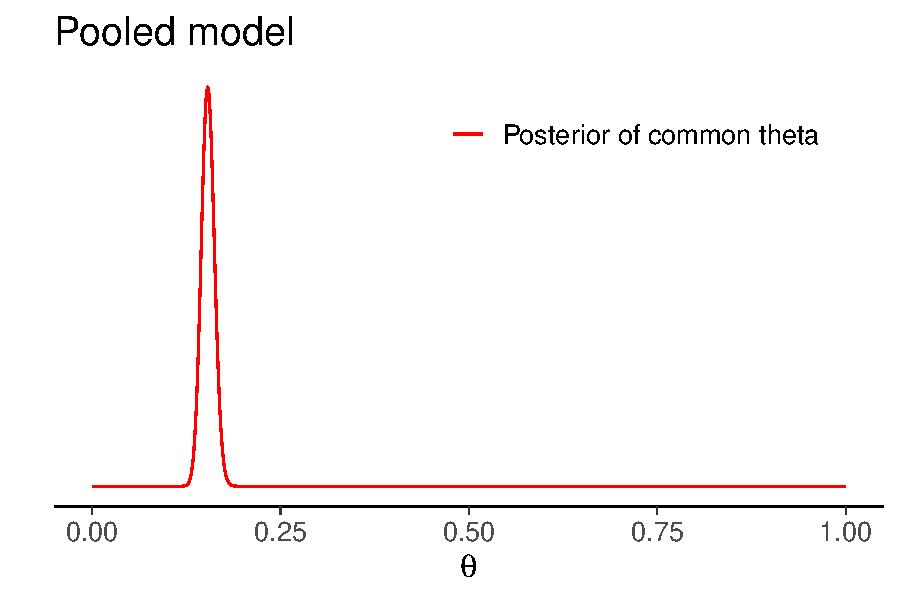
\includegraphics[width=10cm]{rats_pooled.pdf}}
  \only<2>{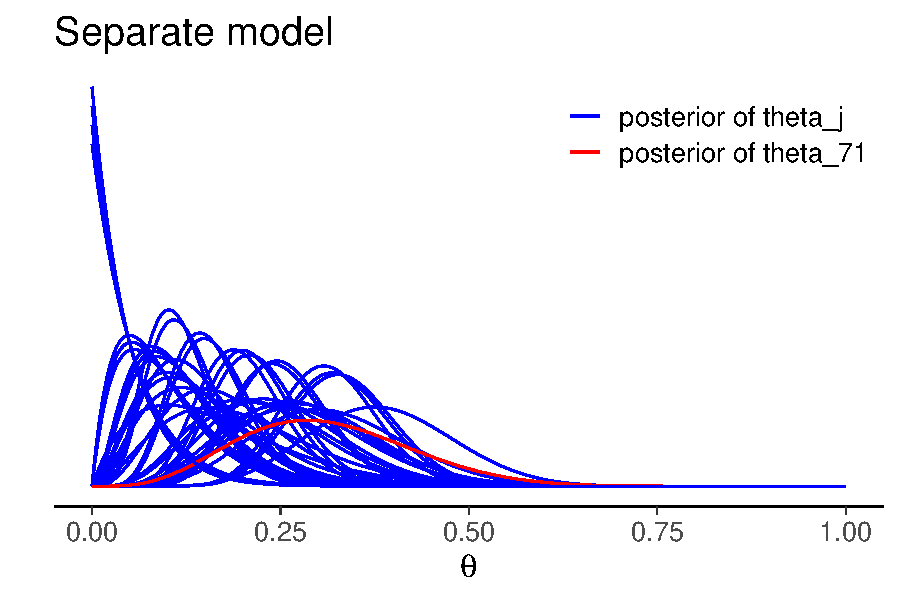
\includegraphics[width=10cm]{rats_separate.pdf}}

  
\end{frame}

\begin{frame}[fragile]
  \frametitle{Hierarchical binomial model: rats}

  \begin{itemize}
  \item Hierarchical binomial model for rats\\
    prior parameters {\color{set11} $\alpha$} and {\color{set11} $\beta$} are unknown
    \begin{minipage}[t]{4cm}
      \xygraph{
        []              !O{y_j}
        ([u]   !V{{\color{set12}\theta_j}}  !P{y_j}
        ([u][l(0.33)] !V{\color{set11} \alpha} !P{{\color{set12}\theta_j}},
        [u][r(0.33)] !V{\color{set11} \beta}  !P{{\color{set12}\theta_j}}),
        [u][r(0.75)]  !F{n_j}    !P{y_j},
        [r(1.0)]*{j},
        [l(3.0)]*{y_j \mid n_j,{\color{set12}\theta_j} \sim \Bin(y_j \mid n_j,{\color{set12}\theta_j})},
        [u][l(2.93)]*{{\color{set12}\theta_j} \mid {\color{set11}\alpha,\beta} \sim
          \Beta({\color{set12}\theta_j} \mid {\color{set11}\alpha,\beta})},
        [l(6.0)]*{~}
        )
        !B{{\color{set12}\theta_j}}{j}{++}
      }
    \end{minipage}
    %\pause
    \item Joint posterior
      $p({\color{set12}\theta_1,\ldots,\theta_J},{\color{set11}\alpha},{\color{set11}\beta} \mid y)$
      \begin{itemize}
    \item multiple parameters
      \pause
      \item factorize
        $\prod_{j=1}^J p({\color{set12}\theta_j} \mid {\color{set11}\alpha,\beta},y)p({\color{set11}\alpha,\beta} \mid y)$
\end{itemize}
\end{itemize}
\end{frame}

\begin{frame}{Hierarchical binomial model: rats}

  \begin{itemize}
  \item Population prior $\Beta({\color{set12}\theta_j} \mid {\color{set11}\alpha,\beta})$
  \item Hyperprior $p({\color{set11}\alpha,\beta})$?
    \begin{itemize}
    \item ${\color{set11}\alpha,\beta}$ both affect the location and scale
    \item BDA3 has
      $p({\color{set11}\alpha,\beta})\propto({\color{set11}\alpha}+{\color{set11}\beta})^{-5/2}$
      \begin{itemize}
      \item diffuse prior for location and scale (BDA3 p. 110)
      \end{itemize}
    \end{itemize}
    \item demo5\_1
    \end{itemize}
\end{frame}

\begin{frame}{Hierarchical binomial model: rats}

  \only<1>{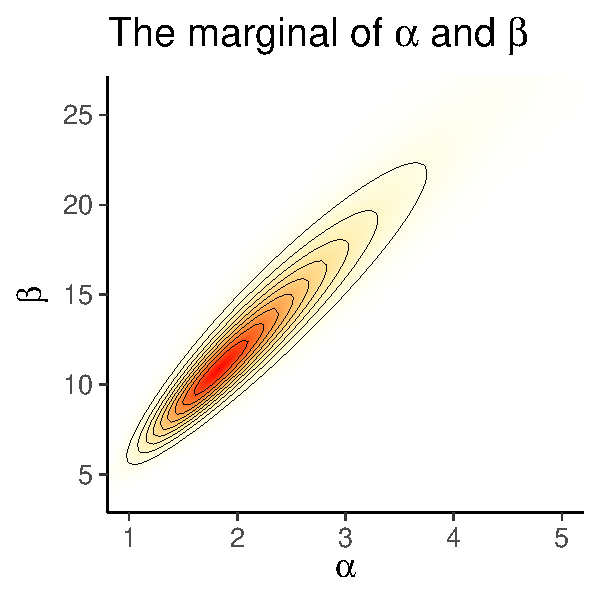
\includegraphics[width=8cm]{rats_posterior.pdf}}
  \only<2>{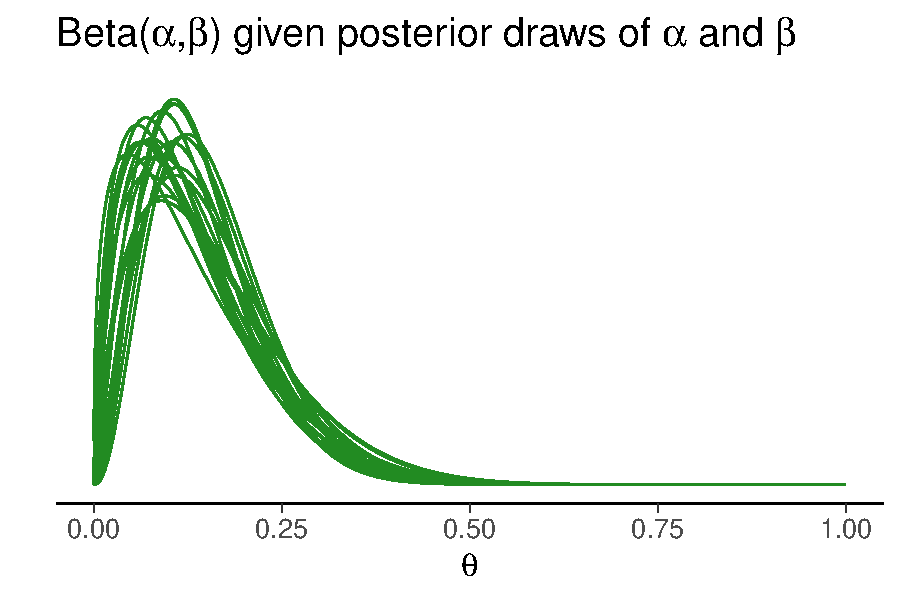
\includegraphics[width=10cm]{rats_hierdraws.pdf}}
  \only<3>{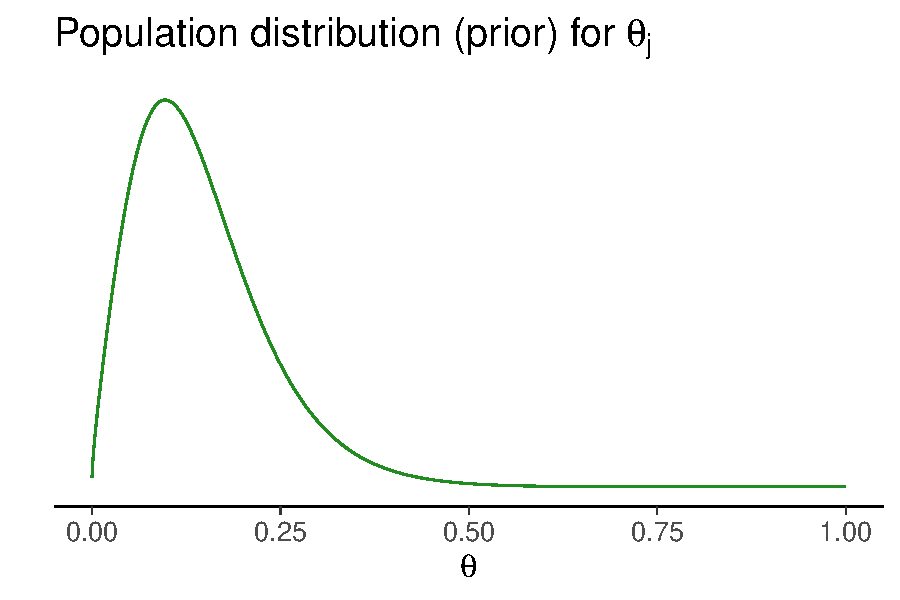
\includegraphics[width=10cm]{rats_hierprior.pdf}}
  \only<4-5>{\vspace{-\baselineskip}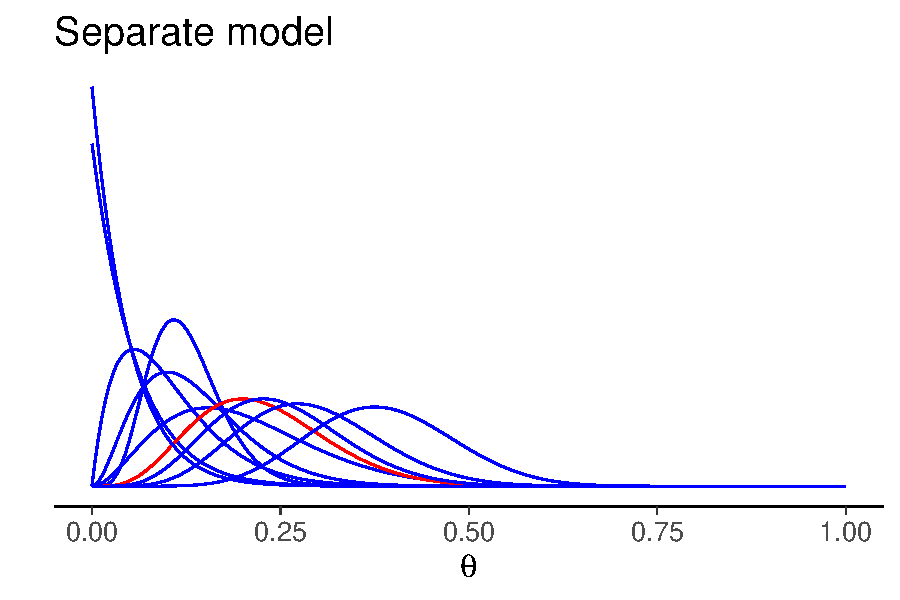
\includegraphics[width=6.7cm]{rats_separate_less.pdf}\\}
  \only<5>{\vspace{-0.3\baselineskip}
    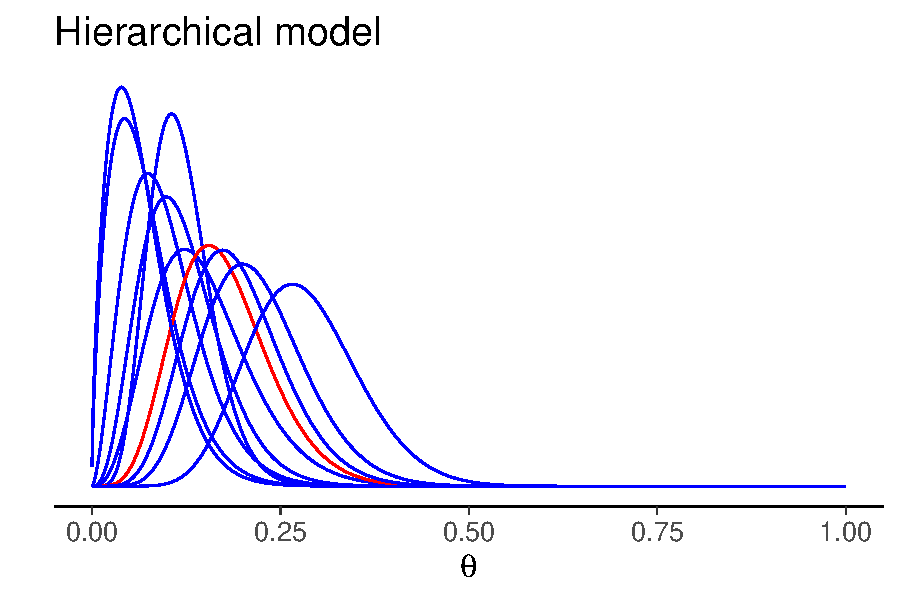
\includegraphics[width=6.7cm]{rats_hier_less.pdf}\\}
  % \only<6>{\vspace{-0.3\baselineskip}
  %   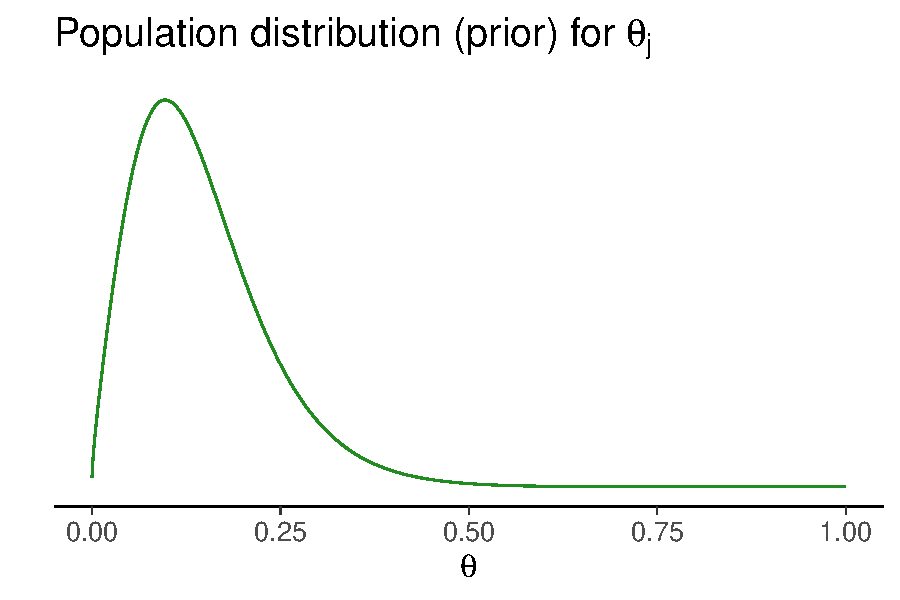
\includegraphics[width=6.7cm]{rats_hierprior.pdf}\\}

\end{frame}

\begin{frame}{Hierarchical model and group size: Rats}

  \vspace{-\baselineskip}
   \begin{minipage}[b]{12cm}
    {  \hspace{-0.7cm}~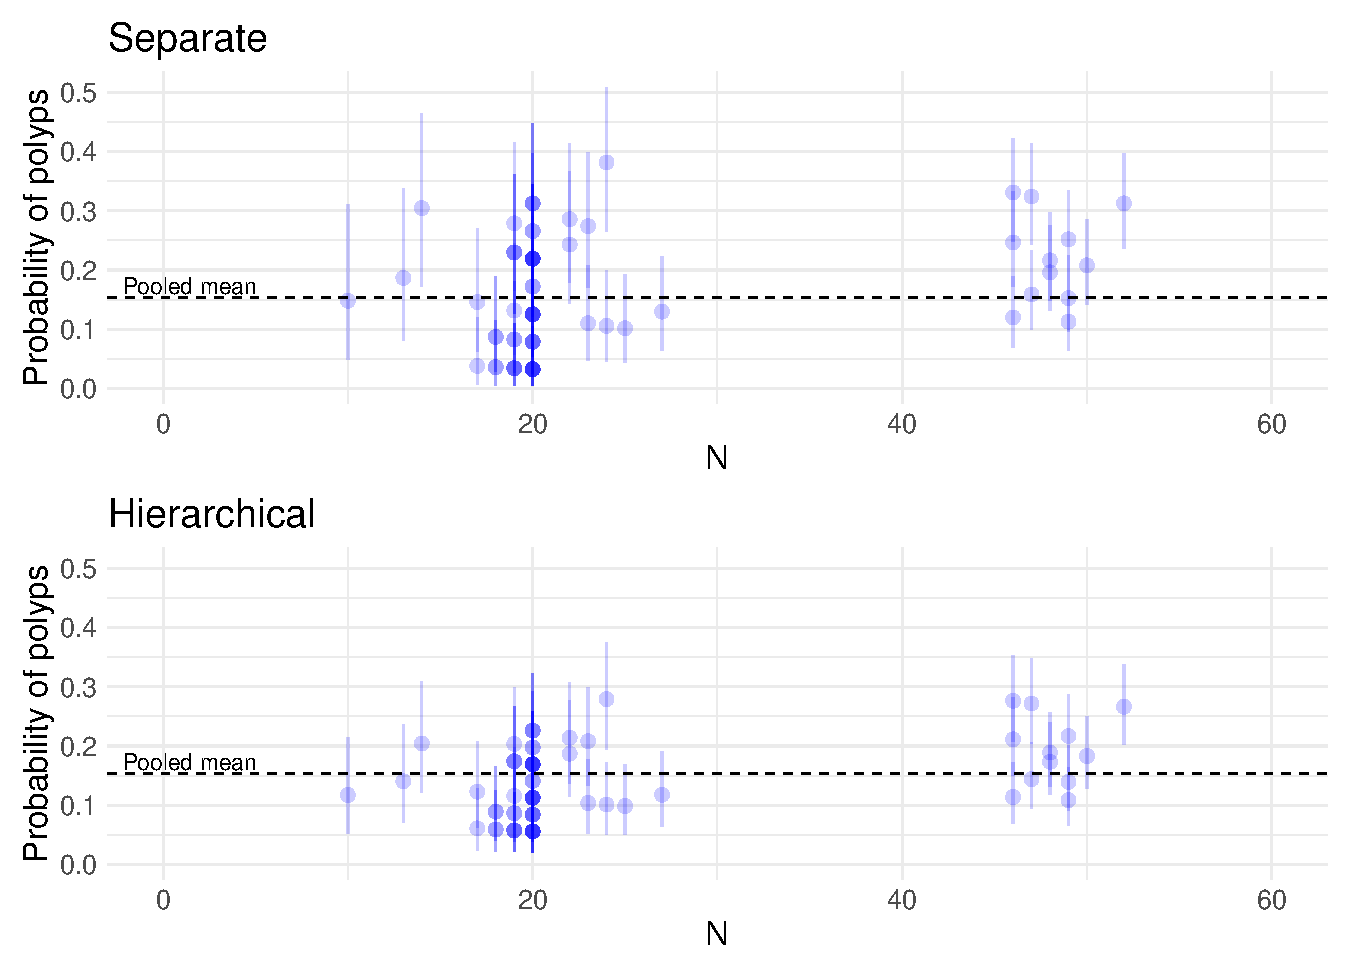
\includegraphics[width=12cm]{rats_shrinkage_size.pdf}}
   \end{minipage}
  
\end{frame}

\begin{frame}{Hierarchical binomial model: rats}

  {\vspace{-\baselineskip}
    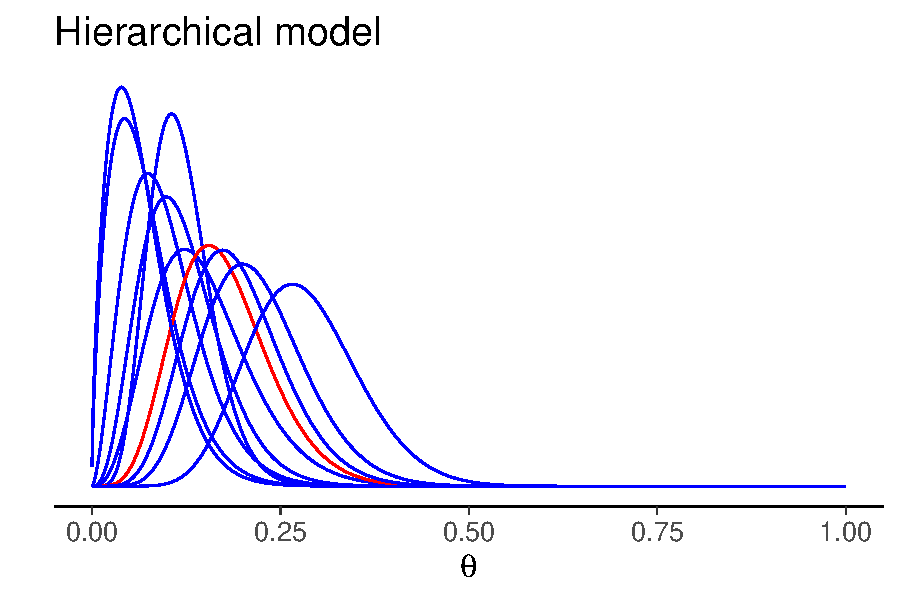
\includegraphics[width=6.7cm]{rats_hier_less.pdf}\\}
  {\vspace{-0.3\baselineskip}
    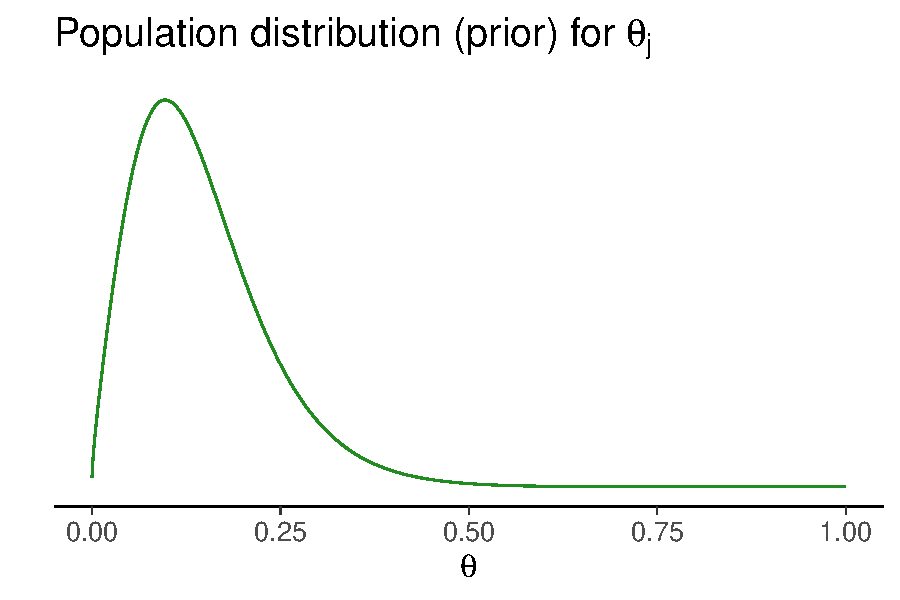
\includegraphics[width=6.7cm]{rats_hierprior.pdf}\\}

\end{frame}

\begin{frame}{Hierarchical model and group size: Radon}

  919 home radon levels in 85 counties in Minnesota:
  
    \hspace{0.2cm} Separate \hspace{4.3cm} Hierarchical
  \begin{minipage}[b]{12cm}
    {  \hspace{-0.9cm}~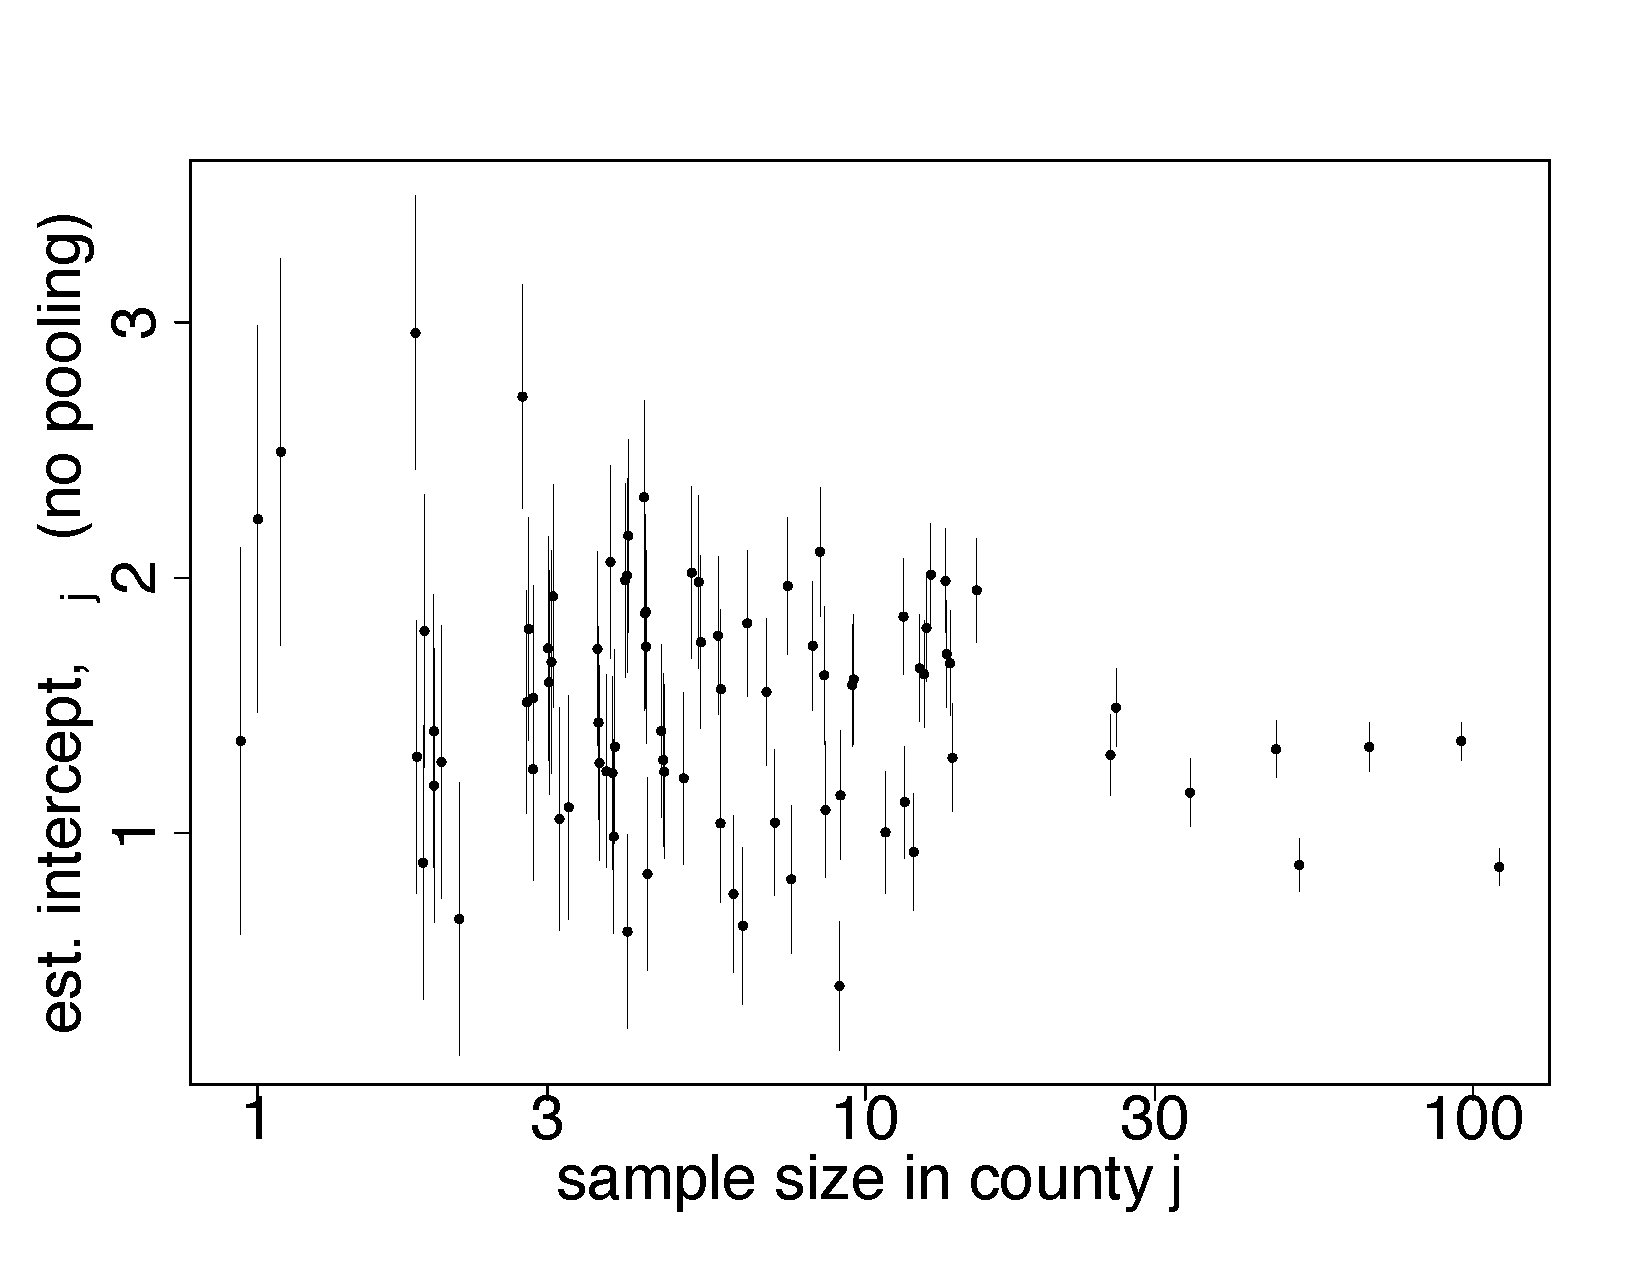
\includegraphics[width=6.3cm]{radon2.pdf}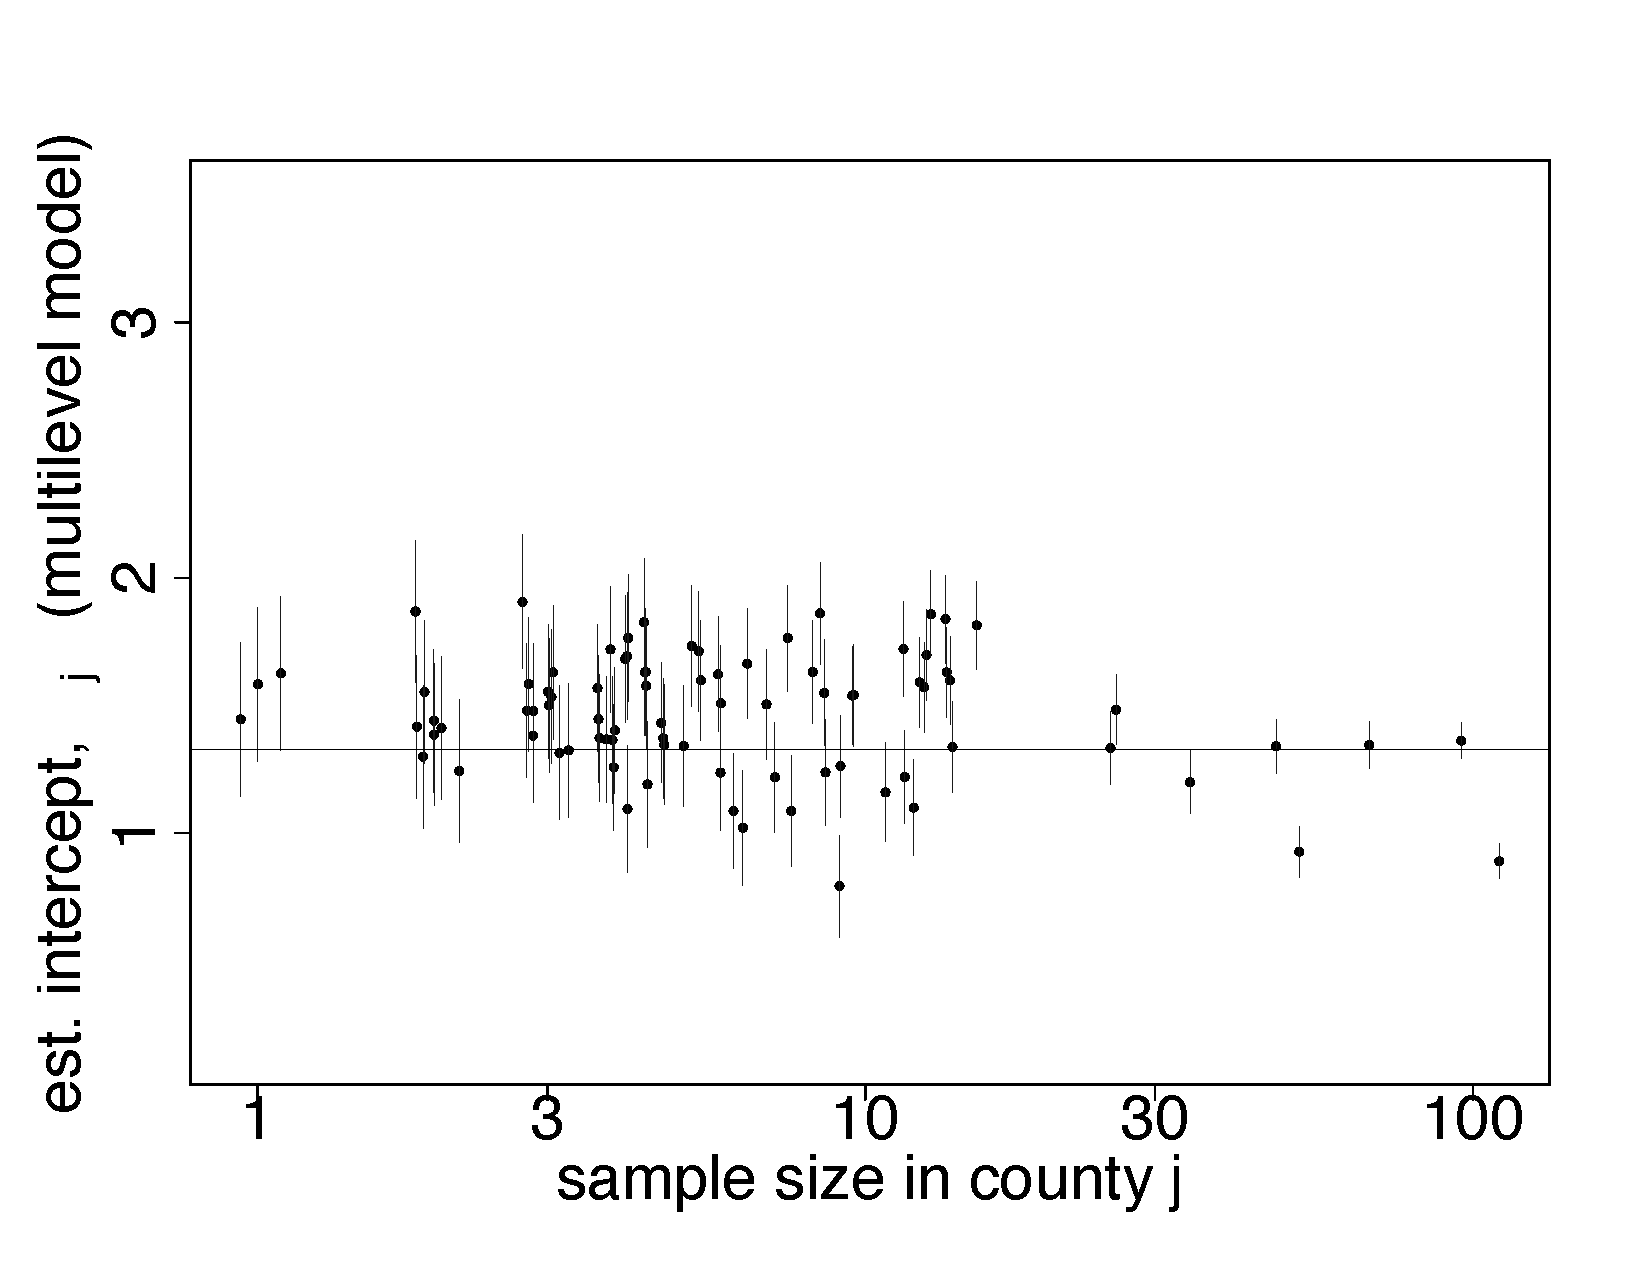
\includegraphics[width=6.3cm]{radon4.pdf}}
  \end{minipage}
  
\end{frame}

\begin{frame}{Diet effect on chicken weights (at age 12 days)}

  \begin{itemize}
  \item A typical treatment effect analysis
  \end{itemize}
  
\end{frame}

\begin{frame}[fragile]{Stan hierarchical model}

  \vspace{-0.5\baselineskip}

\rinline/diet_idx/ is a vector with each element indicating the group

\vspace{-0.5\baselineskip}
{\small
\begin{minted}[highlightlines={10-13}]{stan}
model {
  // Priors
  for (diet in 1:N_diets) {
    mu_diet[diet] ~ normal(mu_0, sd);
  }
  mu_0 ~ normal(0, 1);
  sd ~ normal(0, 1)
  sigma ~ normal(0, 1);
  
  // Observation model
  for (obs in 1:N_observations) {
    weight[obs] ~ normal(mu_diet[diet_idx[obs]], sigma);
  }
}
\end{minted}
}
\end{frame}

\begin{frame}[fragile]{Stan hierarchical model}

  \vspace{-0.5\baselineskip}

\rinline/mu_0/ and \rinline/sd/ are the population mean and sd
  
\vspace{-0.5\baselineskip}
{\small
\begin{minted}[highlightlines={2-5}]{stan}
model {
  // Priors
  for (diet in 1:N_diets) {
    mu_diet[diet] ~ normal(mu_0, sd);
  }
  mu_0 ~ normal(0, 1);
  sd ~ normal(0, 1)
  sigma ~ normal(0, 1);
  
  // Observation model
  for (obs in 1:N_observations) {
    weight[obs] ~ normal(mu_diet[diet_idx[obs]], sigma);
  }
}
\end{minted}
}
\end{frame}

\begin{frame}[fragile]{Stan hierarchical model}

  \vspace{-0.5\baselineskip}

\rinline/sd/ is constrained to be positive and thus the prior is half-normal
  
\vspace{-0.5\baselineskip}
{\small
\begin{minted}[highlightlines={6-7}]{stan}
model {
  // Priors
  for (diet in 1:N_diets) {
    mu_diet[diet] ~ normal(mu_0, sd);
  }
  mu_0 ~ normal(0, 1);
  sd ~ normal(0, 1)
  sigma ~ normal(0, 1);
  
  // Observation model
  for (obs in 1:N_observations) {
    weight[obs] ~ normal(mu_diet[diet_idx[obs]], sigma);
  }
}
\end{minted}
}
\end{frame}

\begin{frame}[fragile]{Stan hierarchical model}

  \vspace{-0.5\baselineskip}

\rinline/sigma/ is constrained to be positive and thus the prior is half-normal
  
\vspace{-0.5\baselineskip}
{\small
\begin{minted}[highlightlines={8}]{stan}
model {
  // Priors
  for (diet in 1:N_diets) {
    mu_diet[diet] ~ normal(mu_0, sd);
  }
  mu_0 ~ normal(0, 1);
  sd ~ normal(0, 1)
  sigma ~ normal(0, 1);
  
  // Observation model
  for (obs in 1:N_observations) {
    weight[obs] ~ normal(mu_diet[diet_idx[obs]], sigma);
  }
}
\end{minted}
}
\end{frame}

\begin{frame}[fragile]{Stan without loops}

  \vspace{-0.5\baselineskip}

  Vectorized statements
  
\vspace{-0.5\baselineskip}
{\small
\begin{minted}[highlightlines={3,9}]{stan}
model {
  // Priors
  mu_diet ~ normal(mu_0, sd);
  mu_0 ~ normal(0, 1);
  sd ~ normal(0, 1)
  sigma ~ normal(0, 1);
  
  // Observation model
  weight ~ normal(mu_diet[diet_idx], sigma);
}
\end{minted}
}

\end{frame}

\begin{frame}[fragile]{Stan vs brms}

  \vspace{-0.5\baselineskip}

  Stan 
  
\vspace{-0.5\baselineskip}
{\small
\begin{minted}{stan}
model {
  // Priors
  mu_diet ~ normal(mu_0, sd);
  mu_0 ~ normal(0, 1);
  sd ~ normal(0, 1)
  sigma ~ normal(0, 1);
  
  // Observation model
  weight ~ normal(mu_diet[diet_idx], sigma);
}
\end{minted}

  brms formula
  \vspace{-0.5\baselineskip}
%\begin{minted}[escapeinside=\%\%,beameroverlays]{r}
\begin{minted}{r}  
brm(weight ~ 1 + (1 | Diet),
\end{minted}
}

\end{frame}

\begin{frame}[fragile]{Stan vs brms}

  \vspace{-0.5\baselineskip}

  Stan
  
\vspace{-0.5\baselineskip}
{\small
\begin{minted}[escapeinside=\%\%]{stan}
model {
  // Priors
  mu_diet ~ normal(mu_0, sd);
  mu_0 ~ normal(0, 1);
  sd ~ normal(0, 1)
  sigma ~ normal(0, 1);
  
  // Observation model
  %\highlight{weight}% ~ normal(mu_diet[diet_idx], sigma);
}
\end{minted}

  brms formula
  \vspace{-0.5\baselineskip}
%\begin{minted}[escapeinside=\%\%,beameroverlays]{r}
\begin{minted}[escapeinside=\%\%]{r}  
brm(%\highlight{weight}% ~ 1 + (1 | Diet),
\end{minted}
}

\end{frame}

\begin{frame}[fragile]{Stan vs brms}

  \vspace{-0.5\baselineskip}

  Stan
  
\vspace{-0.5\baselineskip}
{\small
\begin{minted}[escapeinside=\%\%]{stan}
model {
  // Priors
  mu_diet ~ normal(%\highlight{mu_0}%, sd);
  mu_0 ~ normal(0, 1);
  sd ~ normal(0, 1)
  sigma ~ normal(0, 1);
  
  // Observation model
  weight ~ normal(mu_diet[diet_idx], sigma);
}
\end{minted}

  brms formula
  \vspace{-0.5\baselineskip}
%\begin{minted}[escapeinside=\%\%,beameroverlays]{r}
\begin{minted}[escapeinside=\%\%]{r}  
brm(weight ~%\highlight{ 1 }%+ (1 | Diet),
\end{minted}
}

\end{frame}

\begin{frame}[fragile]{Stan vs brms}

  \vspace{-0.5\baselineskip}

  Stan
  
\vspace{-0.5\baselineskip}
{\small
\begin{minted}[escapeinside=\%\%]{stan}
model {
  // Priors
  %\highlight{mu_diet ~ normal(mu_0, sd)}%;
  mu_0 ~ normal(0, 1);
  sd ~ normal(0, 1)
  sigma ~ normal(0, 1);
  
  // Observation model
  weight ~ normal(mu_diet[diet_idx], sigma);
}
\end{minted}

  brms formula
  \vspace{-0.5\baselineskip}
%\begin{minted}[escapeinside=\%\%,beameroverlays]{r}
\begin{minted}[escapeinside=\%\%]{r}  
brm(weight ~%\highlight{ 1 + (1 | Diet)}%,
\end{minted}
}

\end{frame}

\begin{frame}[fragile]{Stan vs brms}

  \vspace{-0.5\baselineskip}

  Stan
  
\vspace{-0.5\baselineskip}
{\small
\begin{minted}{stan}
model {
  // Priors
  mu_diet ~ normal(mu_0, sd);
  mu_0 ~ normal(0, 1);
  sd ~ normal(0, 1)
  sigma ~ normal(0, 1);
  
  // Observation model
  weight ~ normal(mu_diet[diet_idx], sigma);
}
\end{minted}

  brms formula
  \vspace{-0.5\baselineskip}
\begin{minted}[escapeinside=\%\%]{r}
brm(weight ~ 1 + (1 | Diet), %\highlight{data=Chick12}%,
\end{minted}
}

\end{frame}

\begin{frame}[fragile]{Stan vs brms}

  \vspace{-0.5\baselineskip}

  Stan
  
\vspace{-0.5\baselineskip}
{\small
\begin{minted}[highlightlines={4}]{stan}
model {
  // Priors
  mu_diet ~ normal(mu_0, sd);
  mu_0 ~ normal(0, 1);
  sd ~ normal(0, 1)
  sigma ~ normal(0, 1);
  
  // Observation model
  weight ~ normal(mu_diet[diet_idx], sigma);
}
\end{minted}

  brms formula
  \vspace{-0.5\baselineskip}
\begin{minted}[highlightlines={2}]{r}
brm(weight ~ 1 + (1 | Diet), data=Chick12,
    prior=c(prior(normal(0,1), class="Intercept"), # p(mu_0)
            prior(normal(0,1), class="sd"),        # p(tau)
            prior(normal(0,1), class="sigma")))    # p(sigma)
\end{minted}
}

\end{frame}

\begin{frame}[fragile]{Stan vs brms}

  \vspace{-0.5\baselineskip}

  Stan
  
\vspace{-0.5\baselineskip}
{\small
\begin{minted}[highlightlines={5}]{stan}
model {
  // Priors
  mu_diet ~ normal(mu_0, sd);
  mu_0 ~ normal(0, 1);
  sd ~ normal(0, 1)
  sigma ~ normal(0, 1);
  
  // Observation model
  weight ~ normal(mu_diet[diet_idx], sigma);
}
\end{minted}

  brms formula
  \vspace{-0.5\baselineskip}
\begin{minted}[highlightlines={3}]{r}
brm(weight ~ 1 + (1 | Diet), data=Chick12,
    prior=c(prior(normal(0,1), class="Intercept"), # p(mu_0)
            prior(normal(0,1), class="sd"),        # p(tau)
            prior(normal(0,1), class="sigma")))    # p(sigma)
\end{minted}
}

\end{frame}

\begin{frame}[fragile]{Stan vs brms}

  \vspace{-0.5\baselineskip}

  Stan
  
\vspace{-0.5\baselineskip}
{\small
\begin{minted}[highlightlines={6}]{stan}
model {
  // Priors
  mu_diet ~ normal(mu_0, sd);
  mu_0 ~ normal(0, 1);
  sd ~ normal(0, 1)
  sigma ~ normal(0, 1);
  
  // Observation model
  weight ~ normal(mu_diet[diet_idx], sigma);
}
\end{minted}

  brms formula
  \vspace{-0.5\baselineskip}
\begin{minted}[highlightlines={4}]{r}
brm(weight ~ 1 + (1 | Diet), data=Chick12,
    prior=c(prior(normal(0,1), class="Intercept"), # p(mu_0)
            prior(normal(0,1), class="sd"),        # p(tau)
            prior(normal(0,1), class="sigma")))    # p(sigma)
\end{minted}
}

\end{frame}

\begin{frame}[fragile]{brms generated Stan code}

  \vspace{-\baselineskip}
\begin{minted}[fontsize=\footnotesize,highlightlines={8-10}]{stan}
// generated with brms 2.22.1
data {
  int<lower=1> N;  // total number of observations
  vector[N] Y;  // response variable
  // data for group-level effects of ID 1
  int<lower=1> N_1;  // number of grouping levels
  int<lower=1> M_1;  // number of coefficients per level
  array[N] int<lower=1> J_1;  // grouping indicator per observation
  // group-level predictor values
  vector[N] Z_1_1;
  int prior_only;  // should the likelihood be ignored?
}
\end{minted}
  
\end{frame}

\begin{frame}[fragile]{brms generated Stan code}

  \vspace{-\baselineskip}
\begin{minted}[fontsize=\footnotesize,highlightlines={4-5}]{stan}
parameters {
  real Intercept;  // temporary intercept for centered predictors
  real<lower=0> sigma;  // dispersion parameter
  vector<lower=0>[M_1] sd_1;  // group-level standard deviations
  array[M_1] vector[N_1] z_1;  // standardized group-level effects
}
transformed parameters {
  vector[N_1] r_1_1;  // actual group-level effects
  real lprior = 0;  // prior contributions to the log posterior
  r_1_1 = (sd_1[1] * (z_1[1]));
  lprior += normal_lpdf(Intercept | 0, 1);
  lprior += normal_lpdf(sigma | 0, 1)
    - 1 * normal_lccdf(0 | 0, 1);
  lprior += normal_lpdf(sd_1 | 0, 1)
    - 1 * normal_lccdf(0 | 0, 1);
}
\end{minted}
  
\end{frame}

\begin{frame}[fragile]{brms generated Stan code}

  \vspace{-\baselineskip}
\begin{minted}[fontsize=\footnotesize,highlightlines={11-15}]{stan}
parameters {
  real Intercept;  // temporary intercept for centered predictors
  real<lower=0> sigma;  // dispersion parameter
  vector<lower=0>[M_1] sd_1;  // group-level standard deviations
  array[M_1] vector[N_1] z_1;  // standardized group-level effects
}
transformed parameters {
  vector[N_1] r_1_1;  // actual group-level effects
  real lprior = 0;  // prior contributions to the log posterior
  r_1_1 = (sd_1[1] * (z_1[1]));
  lprior += normal_lpdf(Intercept | 0, 1);
  lprior += normal_lpdf(sigma | 0, 1)
    - 1 * normal_lccdf(0 | 0, 1);
  lprior += normal_lpdf(sd_1 | 0, 1)
    - 1 * normal_lccdf(0 | 0, 1);
}
\end{minted}
  
\end{frame}

\begin{frame}[fragile]{brms generated Stan code}

  \vspace{-\baselineskip}
\begin{minted}[fontsize=\footnotesize,highlightlines={5-10}]{stan}
model {
  // likelihood including constants
  if (!prior_only) {
    // initialize linear predictor term
    vector[N] mu = rep_vector(0.0, N);
    mu += Intercept;
    for (n in 1:N) {
      // add more terms to the linear predictor
      mu[n] += r_1_1[J_1[n]] * Z_1_1[n];
    }
    target += normal_lpdf(Y | mu, sigma);
  }
  // priors including constants
  target += lprior;
  target += std_normal_lpdf(z_1[1]);
}
generated quantities {
  // actual population-level intercept
  real b_Intercept = Intercept;
}
\end{minted}

\end{frame}

\begin{frame}[fragile]{brms generated Stan code}

  \vspace{-\baselineskip}
\begin{minted}[fontsize=\footnotesize,highlightlines={14-15}]{stan}
model {
  // likelihood including constants
  if (!prior_only) {
    // initialize linear predictor term
    vector[N] mu = rep_vector(0.0, N);
    mu += Intercept;
    for (n in 1:N) {
      // add more terms to the linear predictor
      mu[n] += r_1_1[J_1[n]] * Z_1_1[n];
    }
    target += normal_lpdf(Y | mu, sigma);
  }
  // priors including constants
  target += lprior;
  target += std_normal_lpdf(z_1[1]);
}
generated quantities {
  // actual population-level intercept
  real b_Intercept = Intercept;
}
\end{minted}

\end{frame}

% \begin{frame}{Hierarchical normal model: factory}

%   \begin{itemize}
%   \item Factory has 6 machines which quality is evaluated
%   \item Assume hierarchical model
%     \begin{itemize}
%     \item each machine has its own (average) quality $\theta_j$ and
%       common variance $\sigma^2$
%     \end{itemize}
% \begin{minipage}[b]{4cm}
% \begin{xy}
% \xygraph{
%   []              !O{y_{ij}}
%  ([u][l(0.75)]   !V{\theta_j}      !P{y_{ij}}
%  ([u][l(0.33)] !V{\mu_P}      !P{\theta_j},
%    [u][r(0.33)] !V{\sigma_P^2} !P{\theta_j}),
%   [u][r(1.75)]   !V{\sigma^2}   !P{y_{ij}},
%   [r(0.45)]*{i},
%   [r(0.9)]*{j},
% [l(3)]*{y_{ij} \mid \theta_j \sim \N(\theta_j,\sigma^2)},
% [u][l(3)]*{\theta_j \mid \mu_P,\sigma_P^2 \sim \N(\mu_P,\sigma_P^2)},
% )
% !B{y_{ij}}{i}{}
% !B{\theta_j}{j}{++}
%  }
% \end{xy}
%     \end{minipage}
%   \item Can be used to predict the future quality produced by each
%     machine and quality produced by a new similar machine
% %  \item Gibbs sampling exercise later
%   \end{itemize}
% \end{frame}

% \begin{frame}{Hierarchical normal model: factory}

%   \begin{itemize}
%   \item Factory has 6 machines which quality is evaluated
%   \item Assume hierarchical model
%     \begin{itemize}
%     \item each machine has its own (average) quality $\theta_j$ and
%       own variance $\sigma_j^2$
%     \end{itemize}
% \hspace{-1cm}~\begin{minipage}[b]{4cm}
%       \begin{xy}
%         \xygraph{
%           []              !O{y_{ij}}
%           ([u][l(0.75)]   !V{\theta_j}      !P{y_{ij}}
%           ([u][l(0.33)] !V{\mu_P}      !P{\theta_j},
%           [u][r(0.33)] !V{\sigma_P^2} !P{\theta_j}),
%           [u][r(0.75)]   !V{\sigma_j^2}   !P{y_{ij}}
%           ([u][l(0.33)] !V{\sigma_0^2}      !P{\sigma_j^2},
%           [u][r(0.33)] !V{\nu_0} !P{\sigma_j^2}),
%           [r(0.45)]*{i},
%           [r(0.9)]*{j},
%           [l(3.0)]*{y_{ij} \mid \theta_j \sim \N(\theta_j,\sigma_j^2)},
%           [u][l(3.0)]*{\theta_j \mid \mu_P,\sigma_P^2 \sim \N(\mu_P,\sigma_P^2)},
%           [u][r(3.25)]*{\sigma_j^2 \mid \sigma_0^2,\nu_0 \sim \Invchi2(\sigma_0^2,\nu_0)}
%           )
%           !B{y_{ij}}{i}{}
%           !B{\theta_j}{j}{++}
%         }
%       \end{xy}
%     \end{minipage}
%   \item Can be used to predict the future quality produced by each
%     machine and quality produced by a new similar machine
% %  \item Extra points for the Gibbs sampling exercise later
%   \end{itemize}
% \end{frame}

% \begin{frame}{Hierarchical normal model: 8 schools}

%   \begin{itemize}
%   \item Example: SAT coaching effectiveness
%     \begin{itemize}
%     \item in USA commonly used Scholastic Aptitude Test (SAT) is
%       designed so that short term practice should not improve the
%       results significantly
%     \item schools have anyway coaching courses
%     \item test the effectiveness of the coaching courses 
%     \end{itemize}
%     \pause
%   \item SAT
%     \begin{itemize}
%     \item standardized multiple choice test
%     \item mean about 500 and standard deviation about 100
%     \item most scores between 200 and 800
%     \item different topics, e.g., V=Verbal, M=Mathematics
%     \item pre-test PSAT
%     \end{itemize}
% \end{itemize}
% \end{frame}

% \begin{frame}{Hierarchical normal model: 8 schools}

%   \begin{itemize}
%   \item Effectiveness of the SAT coaching
%     \begin{itemize}
%     \item students had made pre-tests PSAT-M and
%       PSAT-V
%     \item part of students were coached
%     \item linear regression was used to estimate the coaching effect
%       $y_j$ for the school $j$ (could be denoted with $\bar{y}_{.j}$,
%       too) and variances $\sigma_j^2$
%     \item $y_j$ approximately normally distributed, with variances
%       assumed to be known based on about 30 students per school
%     \item data is group means and variances (not personal results)
%     \end{itemize}
%     \pause
%   \item Data:
%     {\small
%     \begin{tabular}[t]{r | r r r r r r r r}
%       School & A & B & C & D & E & F & G & H \\
%       $y_j$ & 28 & 8 & -3 & 7 & -1 & 1 & 18 & 12 \\
%       $\sigma_j$ & 15 & 10 & 16 & 11 & 9 & 22 & 20 & 28
%     \end{tabular}}
%   \end{itemize}
% \end{frame}

% \begin{frame}{Hierarchical normal model for group means}

%   \begin{itemize}
%   \item $J$ experiments, unknown $\theta_j$ and known $\sigma^2$
%     \begin{equation*}
%       y_{ij} \mid \theta_j \sim \N(\theta_j,\sigma^2), \quad
%       i=1,\ldots,n_j; \quad j=1,\ldots,J
%     \end{equation*}
%     \vspace{-6mm}
%   \item Group $j$ sample mean and sample variance
%     \begin{eqnarray*}
%       \bar{y}_{.j} & = & \frac{1}{n_j}\sum_{i=1}^{n_j}y_{ij}\\
%       \sigma_j^2 & = & \frac{\sigma^2}{n_j}
%     \end{eqnarray*}
%     \vspace{-6mm}
%     \pause
%   \item Use model
%     \begin{eqnarray*}
%       \bar{y}_{.j} \mid \theta_j \sim \N(\theta_j,\sigma_j^2)
%     \end{eqnarray*}
%      this model can be generalized so that, $\sigma_j^2$ can be
%     different from each other for other reasons than $n_j$
%   \end{itemize}
% \end{frame}

% \begin{frame}{Hierarchical normal model for group means}

%     \begin{minipage}[b]{4cm}
%       \begin{xy}
%         \xygraph{
%           []              !O{\bar{y}_{.j}}
%           ([u][l(0.5)]   !V{\theta_j}      !P{\bar{y}_{.j}}
%           ([u][l(0.33)] !V{\mu}      !P{\theta_j},
%           [u][r(0.33)] !V{\tau} !P{\theta_j}),
%           [u][r(0.5)]   !O{\sigma_j^2}   !P{\bar{y}_{.j}},
%   [r(1.0)]*{j},
%   [l(3.0)]*{\bar{y}_{.j} \mid \theta_j \sim \N(\theta_j,\sigma^2_j)},
%   [u][l(3.0)]*{\theta_j \mid \mu,\tau \sim \N(\mu,\tau^2)}
%   )
%   !B{\theta_j}{j}{++}
% }
% \end{xy}
% \end{minipage}
% \end{frame}

% \begin{frame}{Hierarchical normal model: 8 schools}

%   \only<1-3>{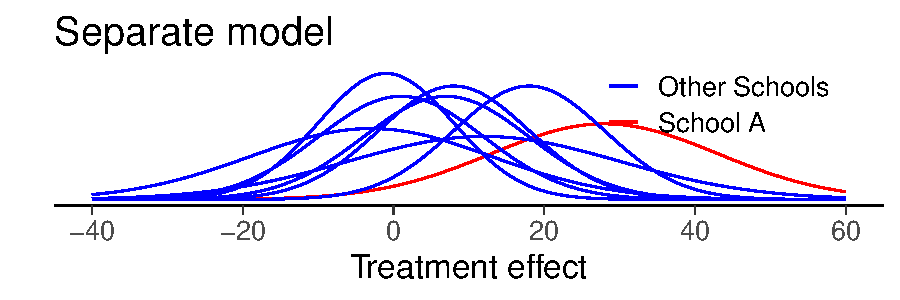
\includegraphics[width=8.3cm]{8schools_separate.pdf}\\}
%   \only<2-3>{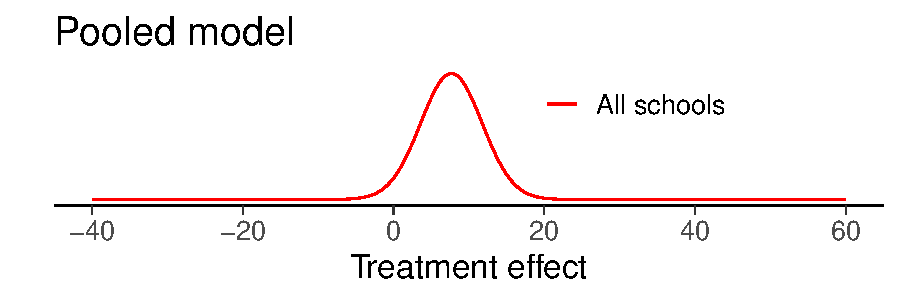
\includegraphics[width=8.3cm]{8schools_pooled.pdf}\\}
%   \only<3>{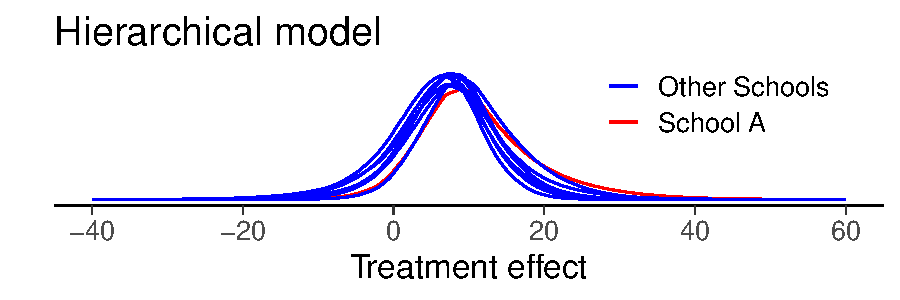
\includegraphics[width=8.3cm]{8schools_hier.pdf}}
%   \only<4-6>{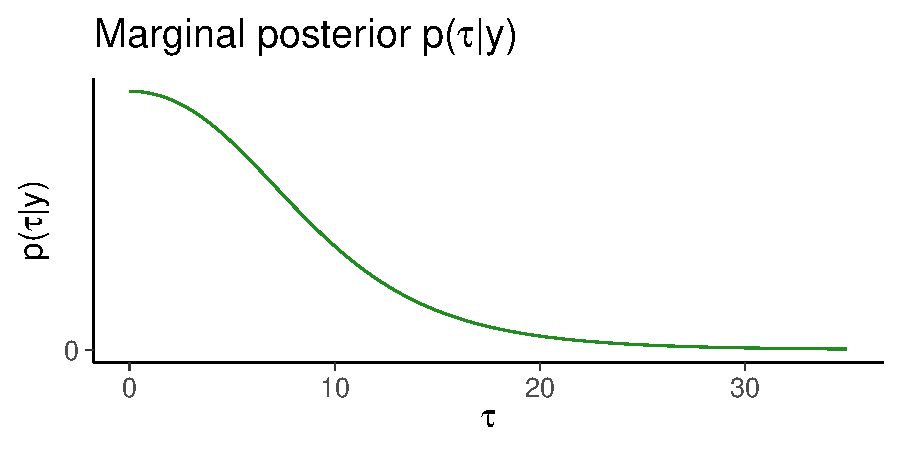
\includegraphics[width=5.5cm]{8schools_tau.pdf}\\}
%   \only<5-6>{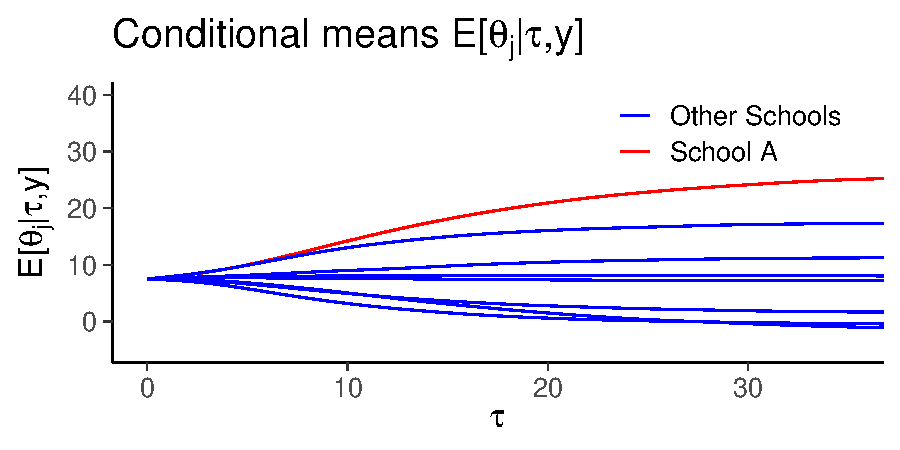
\includegraphics[width=5.5cm]{8schools_condmu.pdf}\\}
%   \only<6>{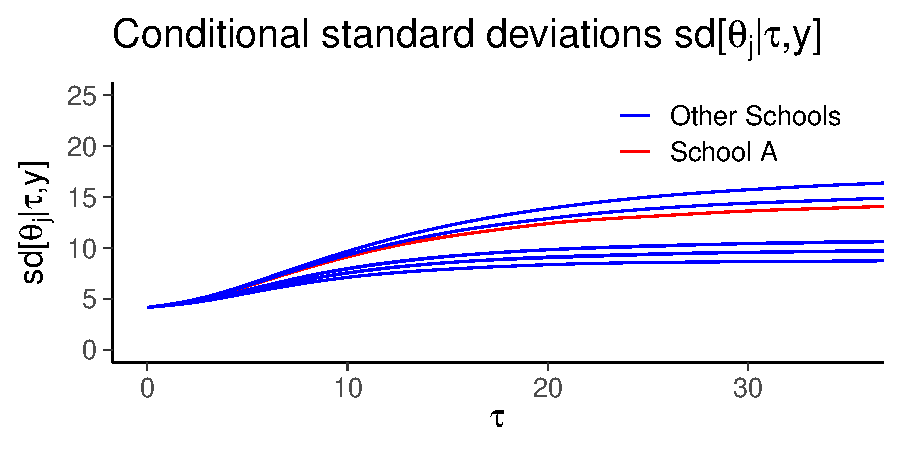
\includegraphics[width=5.5cm]{8schools_condsd.pdf}}
  
% \end{frame}

% \begin{frame}{Paper helicopters}

%   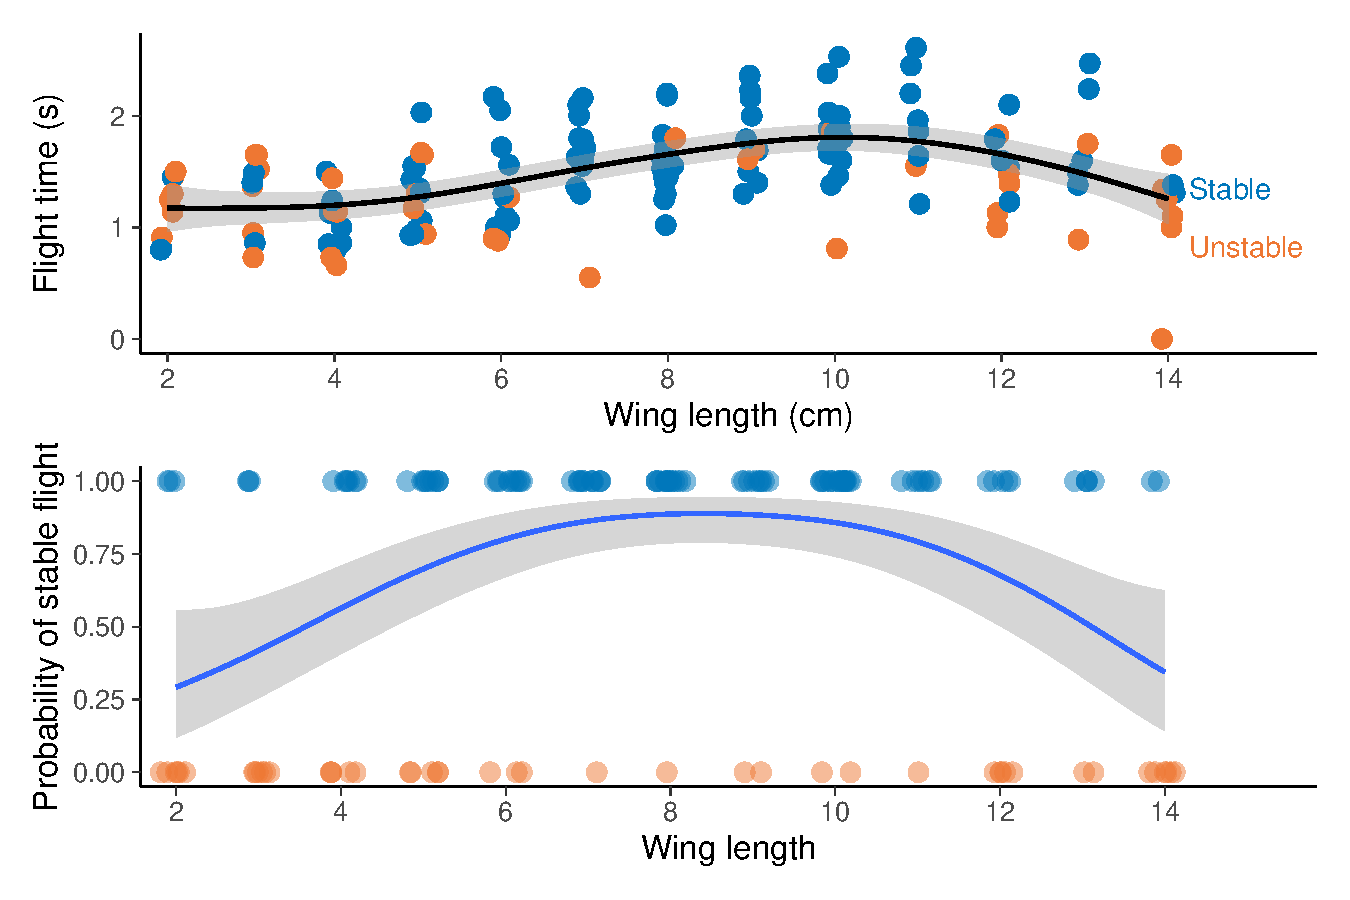
\includegraphics[width=11cm]{helicopter_results.pdf}
  
% \end{frame}

\begin{frame}[fragile]{Paper helicopters: \only<1>{flight time}\only<2>{stability}}

  \vspace{-0.5\baselineskip}
  Separate model vs. hierarchical model
  \vspace{-0.25\baselineskip}
  
  \only<1>{\includegraphics[width=11.5cm]{helicopter_separate_hier_time_2024.pdf}}
  \only<2>{\includegraphics[width=11.5cm]{helicopter_separate_hier_stable_2024.pdf}}
  
\end{frame}

\begin{frame}[fragile]{Paper helicopters: brms}

  Flight time

{\small
\begin{minted}{r}
flight_time ~ s(wing_length) + s(wing_length, by = nclips)
\end{minted}
}

  \includegraphics[width=11.5cm]{helicopter_hier_time_2024.pdf}

\end{frame}

\begin{frame}[fragile]{Paper helicopters: brms}

Stability
  
{\small
\begin{minted}{r}
stable_flight ~ s(wing_length) + s(wing_length, by = nclips),
family = bernoulli()
\end{minted}
}

  \includegraphics[width=11.5cm]{helicopter_hier_stable_2024.pdf}

\end{frame}

\begin{frame}{Student retention}

  Was year 2022 better than earlier year?
  
  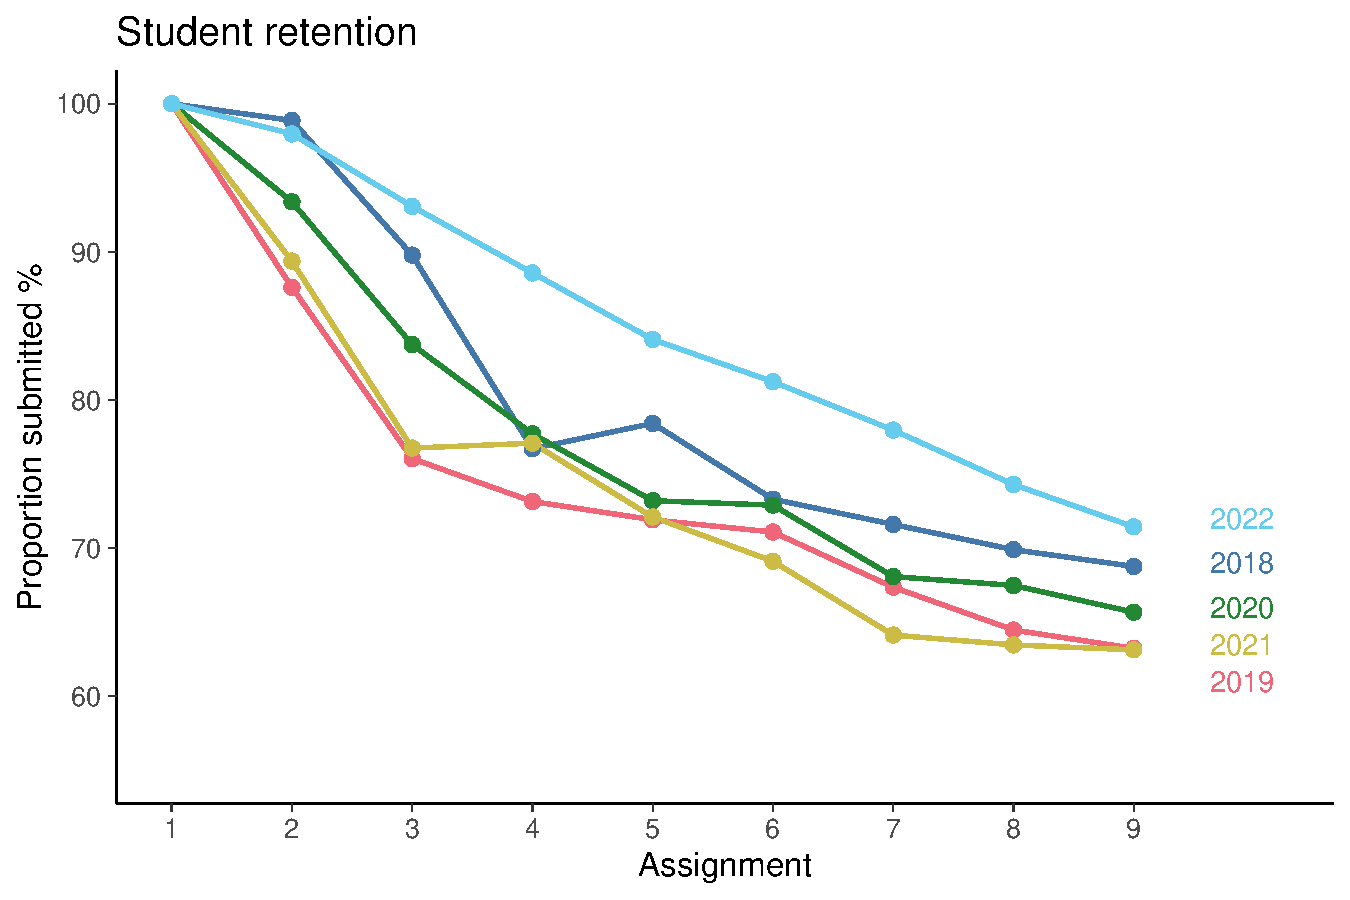
\includegraphics[width=11cm]{student_retention_data.pdf}
  
\end{frame}

\begin{frame}{Student retention \only<1-2>{separate model}\only<3-4>{separate vs hierarchical model}}

  \vspace{-0.75\baselineskip}
  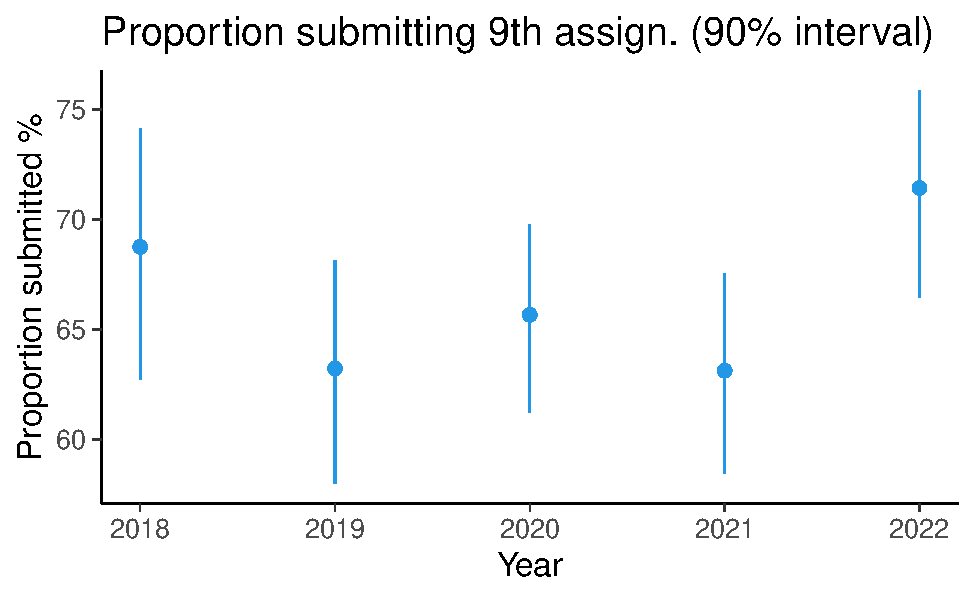
\includegraphics[width=6.8cm]{student_retention_9_binom.pdf}
  \only<2>{\\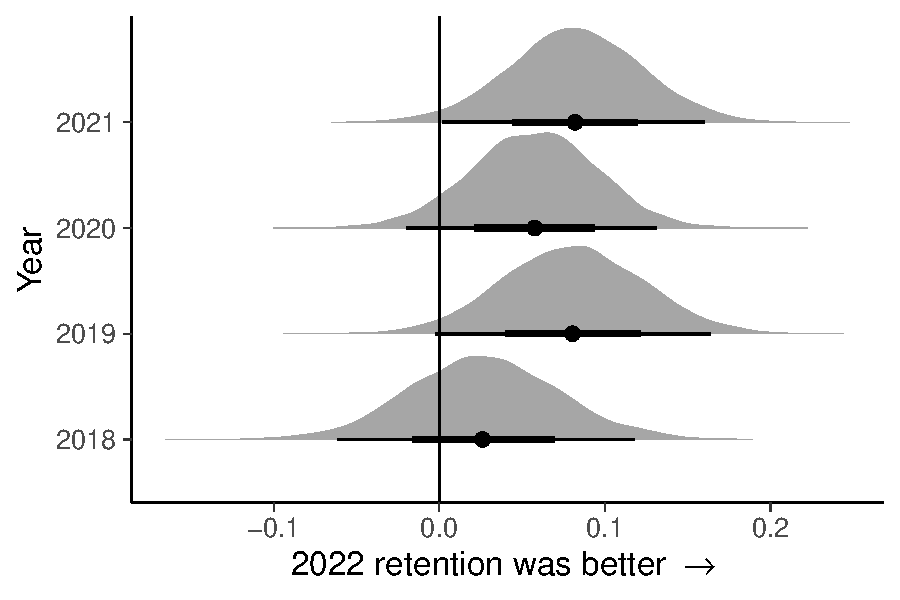
\includegraphics[width=6.3cm]{student_retention_9_binom_comp.pdf}}
  \only<3-4>{\\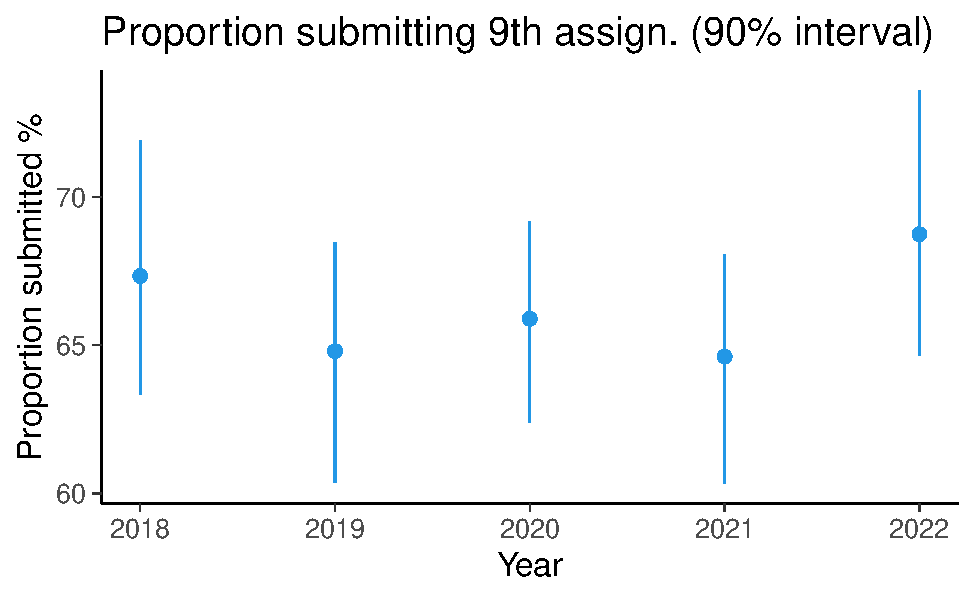
\includegraphics[width=6.6cm]{student_retention_9_binom_hier.pdf}}
  \only<4>{\\\vspace{-0.8\baselineskip}
      \scriptsize \mintinline{r}{nstudents | trials(nstudents1) ~ 1 + (1 | year), family=binomial()}}

\end{frame}

\begin{frame}[fragile]{Student retention latent spline model}

  \vspace{-0.5\baselineskip}
  \hspace{-5mm}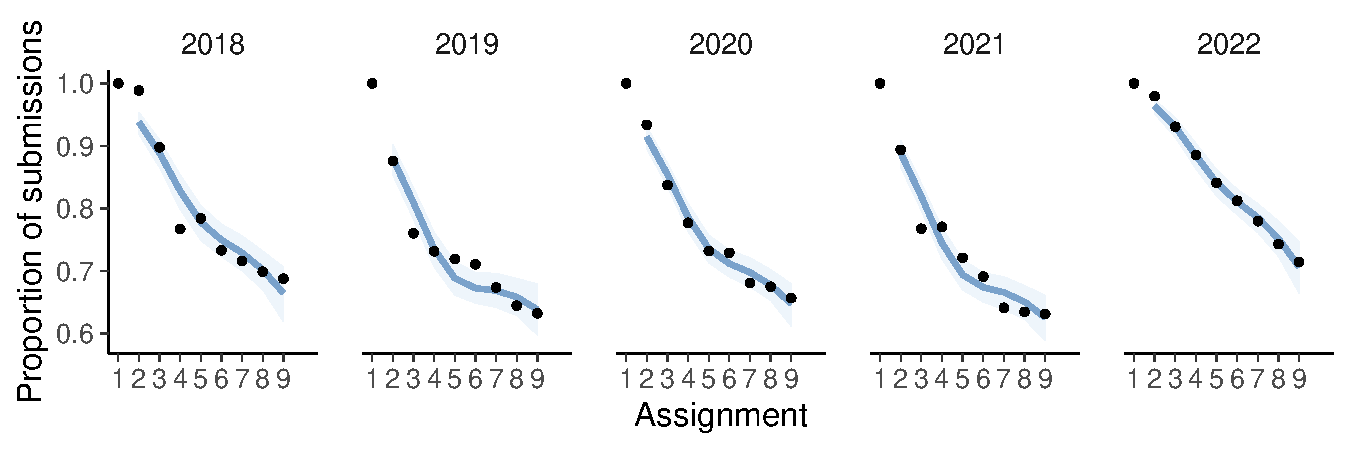
\includegraphics[height=3.6cm]{student_retention_sbinom_linpreds.pdf}
  \only<1>{\\\vspace{-0.5\baselineskip}
    \scriptsize
    \mintinline{r}{nstudents | trials(nstudents1) ~ s(assignment, k=4) + (assignment | year),}~\\~\vspace{-\baselineskip}\\
    \,\,\mintinline{r}{ family=binomial()}
  }
  \begin{minipage}[t][6cm][t]{1.0\linewidth}
    \only<2->{\hspace{-5mm}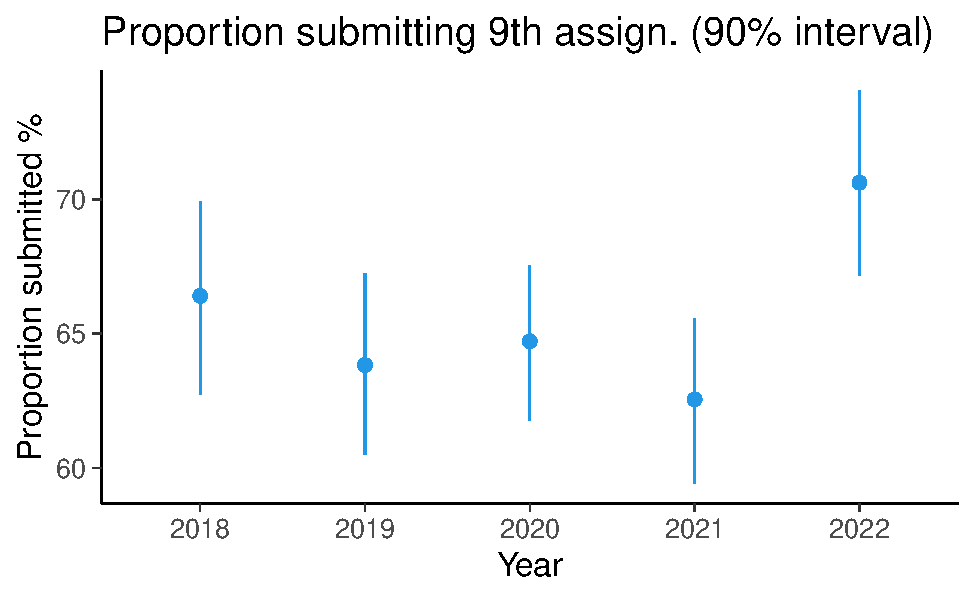
\includegraphics[height=3.7cm]{student_retention_sbinom_hier.pdf}}
    \only<3->{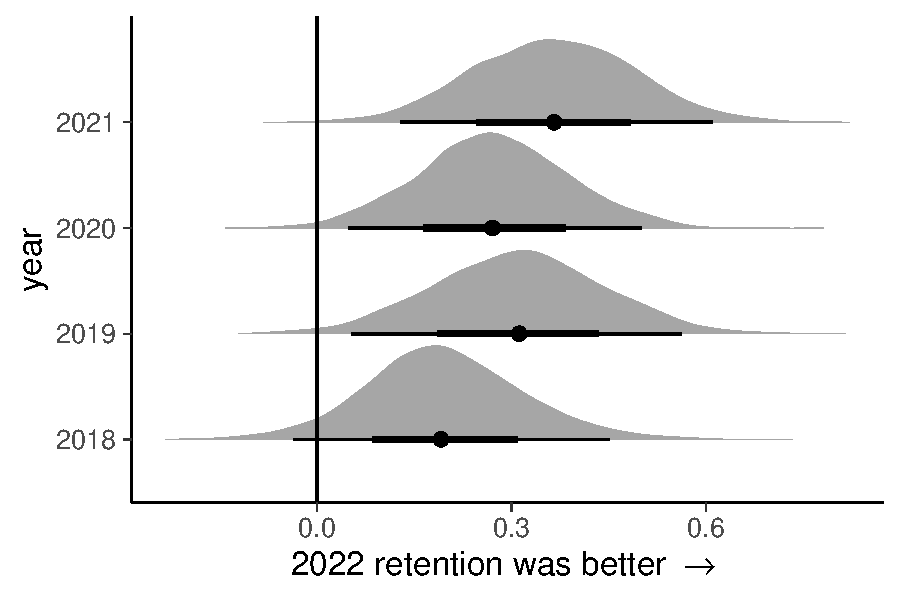
\includegraphics[height=3.4cm]{student_retention_sbinom_hier_comp.pdf}}
  \end{minipage}
\end{frame}

\begin{frame}{Student retention latent spline model, year 2023?}

  \vspace{-0.5\baselineskip}
  \hspace{-8mm}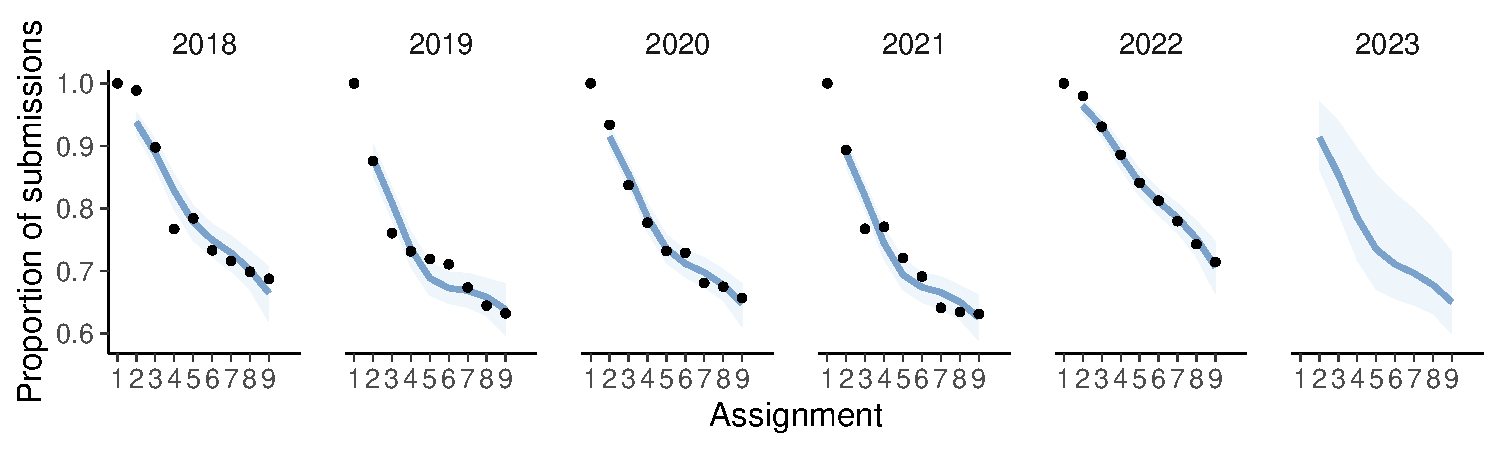
\includegraphics[height=3.5cm]{student_retention_sbinom_linpreds_2.pdf}
  \only<2->{\\\hspace{-5mm}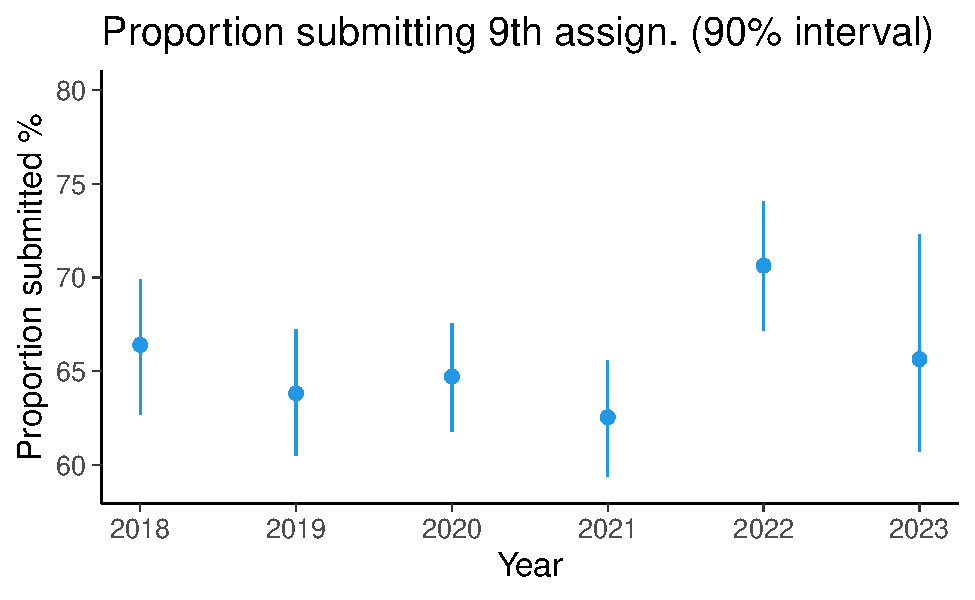
\includegraphics[height=3.7cm]{student_retention_sbinom_hier_2.pdf}}

\end{frame}

\begin{frame}{Student retention latent spline model, year 2023?}

  \vspace{-0.5\baselineskip}
  \hspace{-8mm}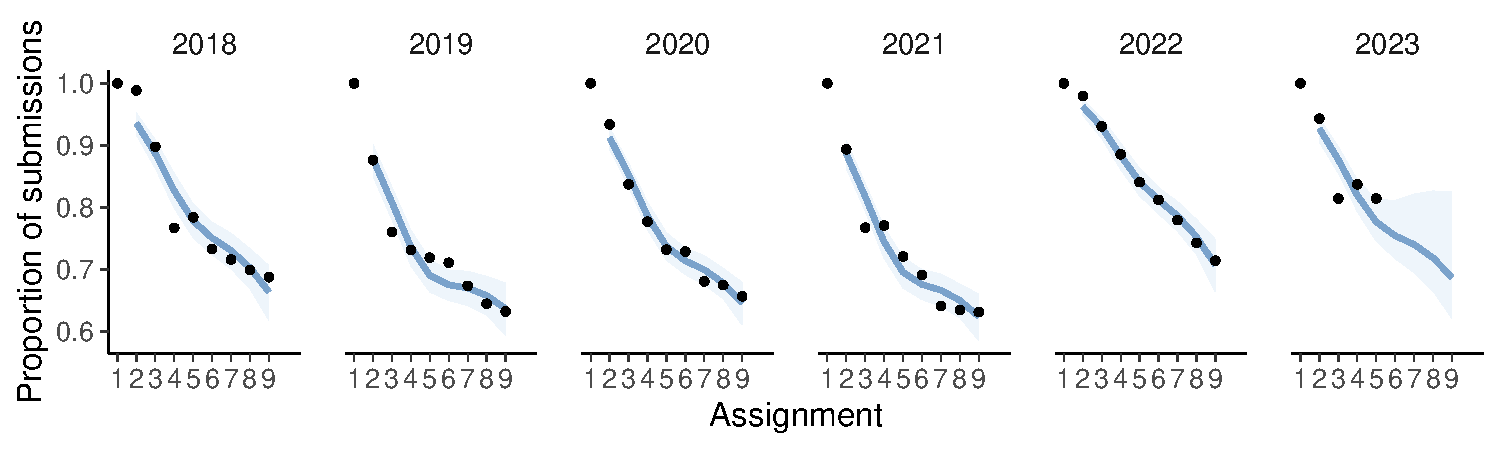
\includegraphics[height=3.5cm]{student_retention_sbinom_linpreds_3.pdf}
  {\\\hspace{-5mm}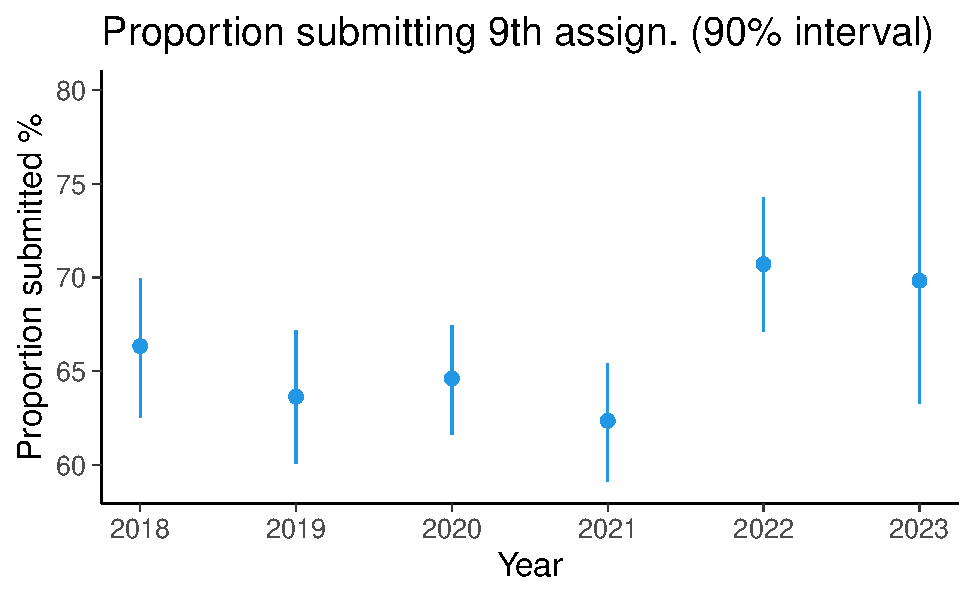
\includegraphics[height=3.7cm]{student_retention_sbinom_hier_3.pdf}}
  \only<2->{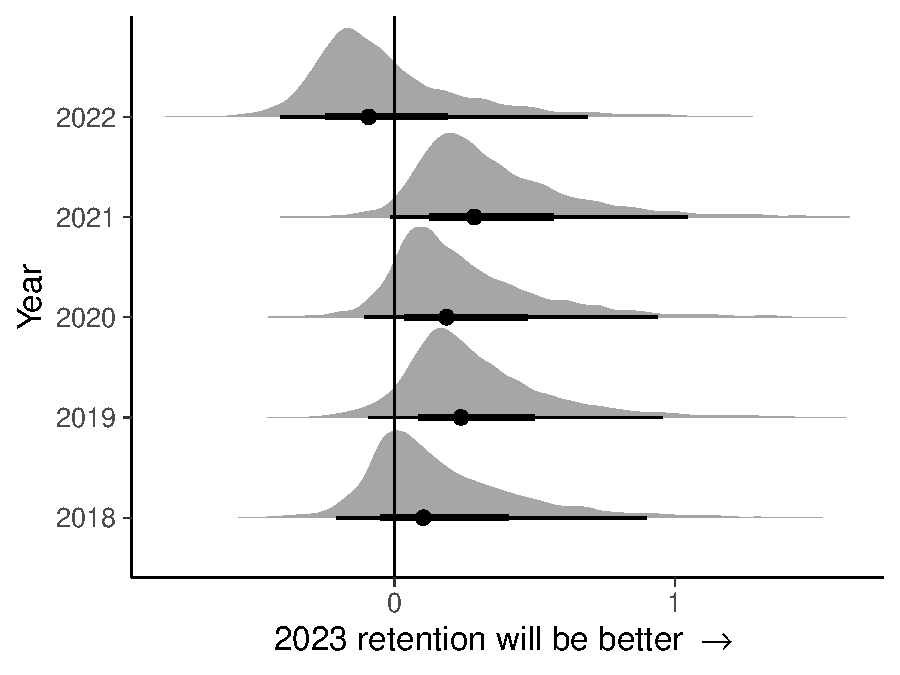
\includegraphics[height=3.4cm]{student_retention_sbinom_hier_comp_3.pdf}}

\end{frame}

\begin{frame}[fragile]{brms summary: one varying coefficient}

  \footnotesize
\rinline/nstudents | trials(nstudents1) ~ 1 + (1 | year), family=binomial()/

\begin{minted}[highlightlines={8-11,13-15},fontsize=\scriptsize,xleftmargin=-5mm]{r}
 Family: binomial 
  Links: mu = logit 
Formula: nstudents | trials(nstudents1) ~ 1 + (1 | year) 
   Data: filter(tb, assignment == 9) (Number of observations: 5) 
  Draws: 4 chains, each with iter = 2000; warmup = 1000; thin = 1;
         total post-warmup draws = 4000

Multilevel Hyperparameters:
~year (Number of levels: 5) 
              Estimate Est.Error l-95% CI u-95% CI Rhat Bulk_ESS Tail_ESS
sd(Intercept)     0.16      0.13     0.01     0.50 1.00      667      878

Regression Coefficients:
          Estimate Est.Error l-95% CI u-95% CI Rhat Bulk_ESS Tail_ESS
Intercept     0.68      0.11     0.45     0.92 1.01      390      242
\end{minted}

\end{frame}

\begin{frame}[fragile]{brms summary: two varying coefficients, nocor}

  \vspace{-0.5\baselineskip}
\begin{minted}[escapeinside=\%\%,fontsize=\footnotesize]{r}
nstudents | trials(nstudents1) ~ assignment + %\highlight{(assignment || year)}%, ...
\end{minted}

\begin{minted}[highlightlines={8-12,14-17},fontsize=\scriptsize,xleftmargin=-5mm]{r}
 Family: binomial 
  Links: mu = logit 
Formula: nstudents | trials(nstudents1) ~ assignment + (assignment || year) 
   Data: filter(tb, assignment > 1) (Number of observations: 40) 
  Draws: 4 chains, each with iter = 2000; warmup = 1000; thin = 1;
         total post-warmup draws = 4000

Multilevel Hyperparameters:
~year (Number of levels: 5) 
               Estimate Est.Error l-95% CI u-95% CI Rhat Bulk_ESS Tail_ESS
sd(Intercept)      0.79      0.45     0.30     1.95 1.00      972     1470
sd(assignment)     0.07      0.06     0.01     0.23 1.01      592      720

Regression Coefficients:
           Estimate Est.Error l-95% CI u-95% CI Rhat Bulk_ESS Tail_ESS
Intercept      2.37      0.38     1.58     3.14 1.01     1114     1471
assignment    -0.21      0.04    -0.30    -0.14 1.00     1056      803
\end{minted}

\end{frame}

\begin{frame}[fragile]{brms summary: two varying coefficients}

  \vspace{-0.5\baselineskip}
\begin{minted}[escapeinside=\%\%,fontsize=\footnotesize]{r}
nstudents | trials(nstudents1) ~ assignment + %\highlight{(assignment | year)}%, ...
\end{minted}

\begin{minted}[highlightlines={8-13},fontsize=\scriptsize,xleftmargin=-5mm]{r}
 Family: binomial 
  Links: mu = logit 
Formula: nstudents | trials(nstudents1) ~ assignment + (assignment | year) 
   Data: filter(tb, assignment > 1) (Number of observations: 40) 
  Draws: 4 chains, each with iter = 2000; warmup = 1000; thin = 1;
         total post-warmup draws = 4000

Multilevel Hyperparameters:
~year (Number of levels: 5) 
                          Estimate Est.Error l-95% CI u-95% CI Rhat Bulk_ESS Tail_ESS
sd(Intercept)                 0.76      0.35     0.34     1.69 1.00     1079     1487
sd(assignment)                0.06      0.03     0.02     0.15 1.00     1211     1979
cor(Intercept,assignment)    -0.85      0.23    -1.00    -0.20 1.00     1730     2265

Regression Coefficients:
           Estimate Est.Error l-95% CI u-95% CI Rhat Bulk_ESS Tail_ESS
Intercept      2.36      0.37     1.60     3.10 1.00      860     1179
assignment    -0.21      0.03    -0.27    -0.14 1.00     1073     1464
\end{minted}

  \pause
  
  brms uses by default multivariate normal population prior for
  multiple varying coefficients, with LKJ prior on the correlation
  matrix
  
\end{frame}

% student_retention_sbinom_hier.pdf
% student_retention_sbinom_hier_comp.pdf

% student_retention_sbinom_hier_2.pdf
% student_retention_sbinom_hier_3.pdf
% student_retention_sbinom_hier_comp_3.pdf

% student_retention_sbinom_linpreds.pdf
% student_retention_sbinom_linpreds_2.pdf
% student_retention_sbinom_linpreds_3.pdf

\begin{frame}[fragile]{Centered vs non-centered parameterization}

\vspace{-0.5\baselineskip}
HMC divergences are more likely when using hierarchical models

\end{frame}

% drop in 2025 vvv
\begin{frame}[fragile]{Divergences}

  \begin{itemize}
  \item HMC specific: indicates that Hamiltonian dynamic simulation
    has problems with unexpected fast changes in log-density
    \begin{itemize}
    \item indicates possibility of biased estimates
    \end{itemize}
  \end{itemize}
     \only<1>{\phantom{\includegraphics[height=5.5cm]{kilpis_hier_cp_hard_trace1.pdf}}}
     \only<2>{\includegraphics[height=5.5cm]{kilpis_hier_cp_hard_trace1.pdf}}
     \only<3>{\includegraphics[height=5.5cm]{kilpis_hier_cp_hard_cummean1.pdf}}
     \only<4>{\includegraphics[height=5.5cm]{kilpis_hier_cp_hard_cummean1b.pdf}}
     \only<5-6>{\includegraphics[height=5.5cm]{kilpis_hier_cp_hard_trace.pdf}}

     \vspace{-1\baselineskip}
     \footnotesize
     \onslide<6>
\begin{minted}{r}
variable  mean median    sd   mad    q5   q95  rhat ess_bulk ess_tail
lsigma0   -1.0   -1.0  0.10 0.070  -1.2 -0.93   1.2      7.2      19.
\end{minted}
     
\end{frame}

\begin{frame}[fragile]{Divergences}

  \begin{itemize}
  \item HMC specific: indicates that Hamiltonian dynamic simulation
    has problems with unexpected fast changes in log-density
    \begin{itemize}
    \item indicates possibility of biased estimates
    \end{itemize}
  \end{itemize}
     \only<1>{\includegraphics[height=5.5cm]{kilpis_hier_cp_hard_trace.pdf}}
     \only<2>{\includegraphics[height=5.5cm]{kilpis_hier_cp_hard_scatter_08.pdf}}
     
     \vspace{-1\baselineskip}
     \footnotesize
\begin{minted}{r}
Warning: 29 of 4000 (1.0%) transitions ended with a divergence.
See https://mc-stan.org/misc/warnings for details.
\end{minted}
     
\end{frame}

\begin{frame}[fragile]{Divergences}

  \begin{itemize}
  \item HMC specific: indicates that Hamiltonian dynamic simulation
    has problems with unexpected fast changes in log-density
    \begin{itemize}
    \item indicates possibility of biased estimates
    \end{itemize}
  \end{itemize}
     \only<1-2>{\includegraphics[height=5.5cm]{kilpis_hier_cp_hard_scatter_08_0999.pdf}}
     \only<3>{\includegraphics[height=5.5cm]{kilpis_hier_cp_0999_hard_trace.pdf}}

     \onslide<2-3>
     \vspace{-1\baselineskip}
     \footnotesize
\begin{minted}{r}
variable  mean median    sd   mad    q5   q95  rhat ess_bulk ess_tail
lsigma0   -1.9   -2.1  0.41  0.13  -2.3 -0.91   2.0      5.8      14.
\end{minted}
     
\end{frame}

\begin{frame}[fragile]{Divergences}

  \begin{itemize}
  \item HMC specific: indicates that Hamiltonian dynamic simulation
    has problems with unexpected fast changes in log-density
    \begin{itemize}
    \item indicates possibility of biased estimates
    \end{itemize}
  \end{itemize}
  \begin{minipage}[t][5cm][t]{1.5\linewidth}
    \hspace{-0.9cm}\includegraphics[height=5cm]{kilpis_hier_cp_ncp_hard_scatter.pdf}
\end{minipage}

     \onslide<2>
     \vspace{-\baselineskip}
     \footnotesize
     With NCP parameterization\\
     \vspace{-1.5\baselineskip}
\begin{minted}{r}
variable  mean median    sd   mad     q5   q95  rhat ess_bulk ess_tail
sigma0    0.27   0.24  0.19  0.20  0.023  0.64   1.0    1571.    1737.
lsigma0  -1.7   -1.4   1.1   0.87 -3.8   -0.45   1.0    1571.    1737.
\end{minted}
     
\end{frame}
% drop in 2025 ^^^

\begin{frame}[fragile]{Centered parameterization}

\vspace{-0.5\baselineskip}
Hierarchical model code from the course demos

{\footnotesize
\begin{minted}{stan}
data {
  int<lower=0> N;                   // number of observations
  int<lower=0> K;                   // number of groups
  array[N] int<lower=1, upper=K> x; // discrete group indicators
  vector[N] y;                      // real valued observations
}
\end{minted}
}
\pause
\vspace{-\baselineskip}
{\footnotesize
\begin{minted}{stan}
parameters {
  real mu0;                         // prior mean
  real<lower=0> sigma0;             // prior std constrained to be pos.
  vector[K] mu;                     // group means
  real<lower=0> sigma;              // common std constrained to be pos.
}
\end{minted}
}
\pause
\vspace{-\baselineskip}
{\footnotesize
\begin{minted}{stan}
model {
  mu0 ~ normal(10, 10);             // weakly informative prior
  sigma0 ~ normal(0, 10);           // weakly informative prior
  mu ~ normal(mu0, sigma0);         // population prior with unknown param.
  sigma ~ lognormal(0, .5);         // weakly informative prior
  y ~ normal(mu[x], sigma);         // observation model
}
\end{minted}
}
\end{frame}

\begin{frame}[fragile]{Centered parameterization}

  First data with many observations per group: 3 summer months with
  each having 71 observations.

  \only<2>{A few divergences that are not clustered.}
  \only<3>{And decreasing step size a little helps.}

  \only<2->{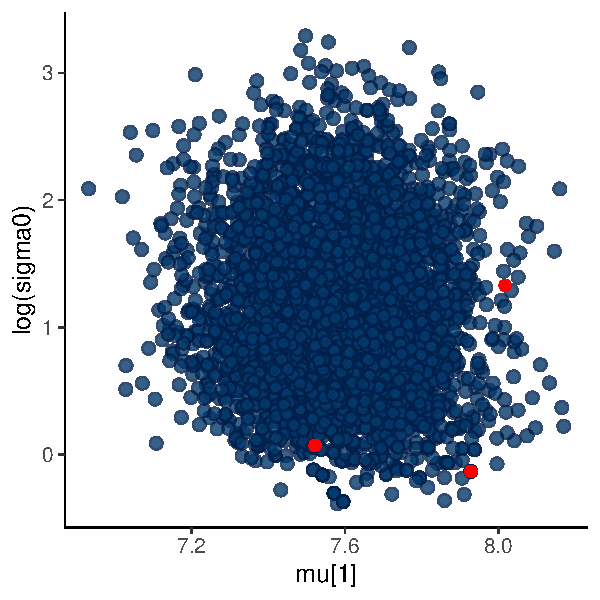
\includegraphics[width=5cm]{kilpis_hier_cp_easy_1.pdf}}
  \only<3>{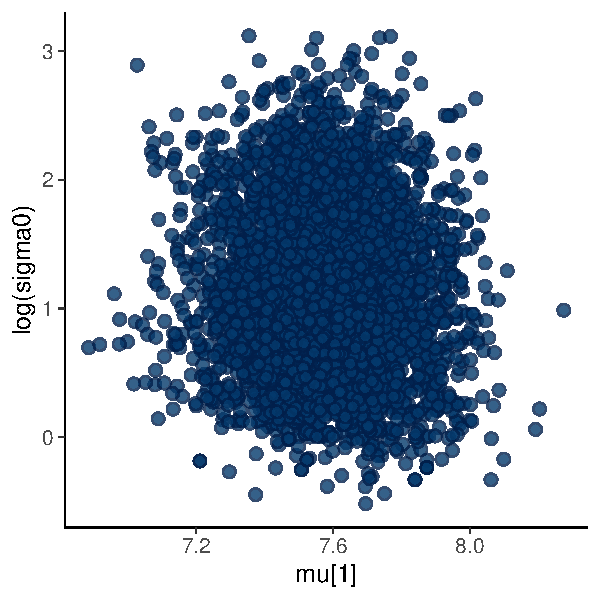
\includegraphics[width=5cm]{kilpis_hier_cp_easy_2.pdf}}
  
\end{frame}

\begin{frame}[fragile]{Centered parameterization}

  Second data with a few observations per group: 71 years with
  each having 3 observations.

  \only<2>{Many divergences that are clustered.}
  \only<3>{And decreasing step size doesn't remove the problem.}

  \only<2->{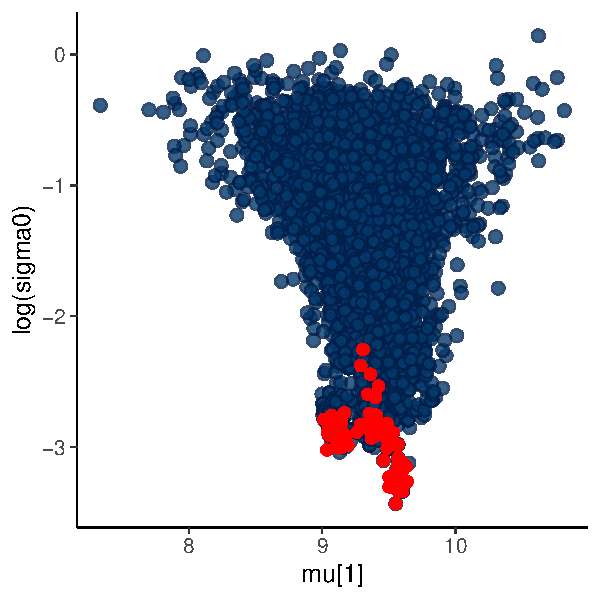
\includegraphics[width=5cm]{kilpis_hier_cp_hard_1.pdf}}
  \only<3>{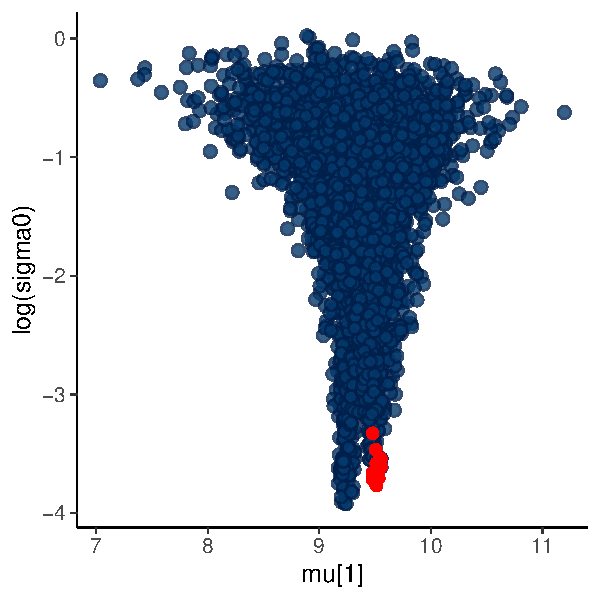
\includegraphics[width=5cm]{kilpis_hier_cp_hard_2.pdf}}
  
\end{frame}

\begin{frame}[fragile]{Centered parameterization}

\vspace{-0.5\baselineskip}
Hierarchical model code from the course demos

\vspace{-\baselineskip}
{\footnotesize
\begin{minted}[highlightlines={4}]{stan}
parameters {
  real mu0;                         // prior mean
  real<lower=0> sigma0;             // prior std constrained to be pos.
  vector[K] mu;                     // group means
  real<lower=0> sigma;              // common std constrained to be pos.
}
\end{minted}
}
\vspace{-\baselineskip}
{\footnotesize
\begin{minted}[highlightlines={4}]{stan}
model {
  mu0 ~ normal(10, 10);             // weakly informative prior
  sigma0 ~ normal(0, 10);           // weakly informative prior
  mu ~ normal(mu0, sigma0);         // population prior with unknown param.
  sigma ~ lognormal(0, .5);         // weakly informative prior
  y ~ normal(mu[x], sigma);         // observation model
}
\end{minted}
}
\end{frame}

\begin{frame}[fragile]{Non-centered parameterization}

\vspace{-0.5\baselineskip}
Transformation

{\footnotesize
\begin{minted}[highlightlines=4]{stan}
parameters {
  real mu0;                         // prior mean
  real<lower=0> sigma0;             // prior std constrained to be pos.
  vector[K] z;                      // latent variable
  real<lower=0> sigma;              // common std constrained to be pos.
}
\end{minted}
}
\vspace{-\baselineskip}
{\footnotesize
\begin{minted}[highlightlines=2]{stan}
transformed parameters {
  vector[K] mu = mu0 + sigma0 * z;  // group means
}
\end{minted}
}
\vspace{-\baselineskip}
{\footnotesize
\begin{minted}[highlightlines=4]{stan}
model {
  mu0 ~ normal(10, 10);     // weakly informative prior
  sigma0 ~ normal(0, 10);   // weakly informative prior
  z ~ normal(0, 1);         // unit normal
  sigma ~ lognormal(0, .5); // weakly informative prior
  y ~ normal(mu[x], sigma); // observation model
}
\end{minted}
}

\end{frame}

\begin{frame}[fragile]{Non-centered parameterization}

  Second data with a few observations per group: 71 years with
  each having 3 observations.

  \only<2>{A few divergences that are not clustered.}
  \only<3>{And decreasing step size a little helps.}
  \only<4>{Because we're actually sampling \texttt{z} and not \texttt{mu}}

  \only<2->{\includegraphics[width=5cm]{kilpis_hier_ncp_hard_1.pdf}}
  \only<3>{\includegraphics[width=5cm]{kilpis_hier_ncp_hard_2.pdf}}
  \only<4>{\includegraphics[width=5cm]{kilpis_hier_ncp_hard_z_2.pdf}}
  
\end{frame}

\begin{frame}[fragile]{Non-centered parameterization}

  No free lunch

  \begin{itemize}
  \item non-centered parameterization is good when likelihood is weak
  \item non-centered parameterization is bad when likelihood is strong
  \end{itemize}
  
\end{frame}

\begin{frame}[fragile]{Non-centered parameterization}

  First data with many observations per group: 3 summer months with
  each having 71 observations.

  \only<2>{Many divergences that are not clustered.}
  \only<3>{But decreasing step size a lot helps.}
  \only<4>{Now the posterior for \texttt{z} is problematic.}

  \only<2->{\includegraphics[width=5cm]{kilpis_hier_ncp_easy_1.pdf}}
  \only<3>{\includegraphics[width=5cm]{kilpis_hier_ncp_easy_2.pdf}}
  \only<4>{\includegraphics[width=5cm]{kilpis_hier_ncp_easy_z_1.pdf}}
  
\end{frame}

\begin{frame}[fragile]{Centered vs. non-centered parameterization}

  \vspace{-1\baselineskip}
  \hspace{15mm} Strong likelihood \hspace{14mm} Weak likelihood\\
  \hspace{10mm}{\includegraphics[width=4cm]{kilpis_hier_cp_easy_2.pdf}}
  {\includegraphics[width=4cm]{kilpis_hier_cp_hard_1.pdf}}\\
  \hspace{10mm}{\includegraphics[width=4cm]{kilpis_hier_ncp_easy_1.pdf}}
  {\includegraphics[width=4cm]{kilpis_hier_ncp_hard_2.pdf}}\\
  \vspace{-80mm}\rotatebox{90}{Non-centered param. \hspace{8mm} Centered param. }
  
\end{frame}

\begin{frame}[fragile]{brms and rstanarm}

  \begin{itemize}
  \item<+-> brms and rstanarm use non-centered parameterization
    \begin{itemize}
    \item as hierarchical models and Bayesian inference is most useful
      when likelihood is weak
    \end{itemize}
  \item<+-> If the likelihood is highly informative for all groups, and
    the non-centered parameterization is causing divergences,
    \begin{itemize}
    \item use fixed population prior model as the hierarchical part is not
      that important with strong likelihood. Instead of 
\begin{minted}[fontsize=\footnotesize]{r}
y ~ 1 + (1 | group)
\end{minted}
      use, for example, 
\begin{minted}[fontsize=\footnotesize]{r}
y ~ 1 + group,
prior = prior(normal(0, 10), class='b')
\end{minted}
    \end{itemize}
  \item<+-> There can be need for both centered and non-centered
    parameterization in the same model
    \begin{itemize}
    \item automation not easy, but research goes on
    \end{itemize}
  \end{itemize}
\end{frame}

\begin{frame}[fragile]{brms non-centered parameterization}

  \vspace{-\baselineskip}
\begin{minted}[fontsize=\footnotesize,highlightlines={5,8,9,16,19},mathescape]{stan}
parameters {
  real Intercept;  // temporary intercept for centered predictors
  real<lower=0> sigma;  // dispersion parameter
  vector<lower=0>[M_1] sd_1;  // group-level standard deviations
  array[M_1] vector[N_1] z_1;  // standardized group-level effects
}
transformed parameters {
  vector[N_1] r_1_1;  // actual group-level effects
  r_1_1 = (sd_1[1] * (z_1[1]));
//...
}
model {
//...
    for (n in 1:N) {
      // add more terms to the linear predictor
      mu[n] += r_1_1[J_1[n]] * Z_1_1[n];
    }
//...
  target += std_normal_lpdf(z_1[1]);
}
\end{minted}

\end{frame}

\begin{frame}[fragile]{Kilpisjärvi summer temperature}
  
  Posterior draws of alpha and beta
  
  \begin{center}
    \includegraphics[width=10cm]{kilpis_lin_mcmc_scatter.pdf}
  \end{center}

\scriptsize
\begin{minted}{r}
Warning: 1 of 4000 (0.0%) transitions hit the maximum treedepth limit of 10.
See https://mc-stan.org/misc/warnings for details.
\end{minted}
\pause
\small
Solution was to center the covariate time to have mean 0, so that the
intercept is the expected temperature in the middle of the range
  
\end{frame}

\begin{frame}[fragile,fragile]{brms covariate centering by default}

  \vspace{-0.75\baselineskip}
\begin{minted}[fontsize=\footnotesize]{r}
fit_lin <- brm(temp ~ year, data = data_lin)
\end{minted}
\pause
\begin{minted}[fontsize=\scriptsize,highlightlines={5,6,11,16,21}]{r}
transformed data {
  matrix[N, Kc] Xc;  // centered version of X without an intercept
  vector[Kc] means_X;  // column means of X before centering
  for (i in 2:K) {
    means_X[i - 1] = mean(X[, i]);
    Xc[, i - 1] = X[, i] - means_X[i - 1];
  }
}
parameters {
  vector[Kc] b;  // regression coefficients
  real Intercept;  // temporary intercept for centered predictors
  real<lower=0> sigma;  // dispersion parameter
}
model {
//...
  target += normal_id_glm_lpdf(Y | Xc, Intercept, b, sigma);
//...
}
generated quantities {
  // actual population-level intercept
  real b_Intercept = Intercept - dot_product(means_X, b);
}
\end{minted}

\end{frame}

\begin{frame}[fragile,fragile]{brms covariate centering by default}

  Sometimes we want to turn off the covariate centering, which can be
  done with additional argument for brms formula function
  \rinline/bf()/

\begin{minted}[fontsize=\footnotesize,escapeinside=\%\%]{r}
fit_lin <- brm(%\highlight{bf(temp ~ year, center=FALSE)}%, data = data_lin)
\end{minted}

\end{frame}

\begin{frame}[fragile]{brms formulas}

  \begin{tabular}[t]{lll}
    model & formula & alternative formula \\ \hline
    intercept only & & \\
    $y \sim \N(\alpha, \sigma)$ & \rinline/y ~ 1/ & \\\pause
    linear models & & \\
  $y \sim \N(\alpha + \beta x, \sigma)$ & \rinline/y ~ x/ & \rinline/y ~ 1 + x/ \\\pause
  $y \sim \N(\beta x, \sigma)$ & \rinline/y ~ 0 + x/ & \rinline/y ~ -1 + x/ \\ \pause
     hierarchical models  && \\
  $y \sim \N(\alpha_0 + \alpha_g + \beta x, \sigma)$ & \rinline/y ~ x + (1 | g)/ & \\\pause
  $y \sim \N(\alpha_0 + \alpha_g + \beta_0 x + \beta_g x, \sigma)$ & \rinline/y ~ x + (x | g)/ & (see above) \\
  \end{tabular}

\end{frame}

\begin{frame}[fragile]{brms formulas}

  \begin{tabular}[t]{lll}
    model & formula \\ \hline
    heteroskedastic & \\
    $y \sim \N\left(\alpha_\mu + \beta_\mu x,\, \exp(\alpha_\sigma + \beta_\sigma x)\right)$ & \rinline/bf(y ~ x, sigma ~ x)/ \\
  \end{tabular}

\end{frame}

\begin{frame}[fragile]{brms families}

  \rinline/family/ argument determines the observation model family

  \small
  \begin{tabular}[t]{lll}
    model & brms \\ \hline
    $y \sim t_{\nu}(\alpha + \beta x, \sigma)$ & \rinline/y ~ x, family = student()/  \\
    $y \sim \Bin(\logit^{-1}(\alpha + \beta x), N)$ & \rinline/y | trials(N) ~ x, family = binomial()/  \\
    $y \sim \Negbin(\exp(\alpha + \beta x), \phi)$ & \rinline/y ~ x, family = negbinomial()/  \\
  \end{tabular}

  
\end{frame}

\begin{frame}[fragile]{Meta-analysis}
\framesubtitle{Pharmacologic treatments for chronic obstructive pulmonary disease}

\begin{minted}[fontsize=\footnotesize]{r}
> head(dat.baker2009)
                  study year id   treatment exac total
1 Llewellyn-Jones 1996 1996  1 Fluticasone    0     8
2 Llewellyn-Jones 1996 1996  1     Placebo    3     8
3            Boyd 1997 1997  2  Salmeterol   47   229
4            Boyd 1997 1997  2     Placebo   59   227
5        Paggiaro 1998 1998  3 Fluticasone   45   142
6        Paggiaro 1998 1998  3     Placebo   51   139
\end{minted}
  
\end{frame}

\begin{frame}[fragile]{Meta-analysis}
\framesubtitle{Pharmacologic treatments for chronic obstructive pulmonary disease}

\only<1>{A big variation in the number of patients per study}
\only<2>{2--4 drugs tested per study, and some not including placebo}

\begin{minipage}[t][][t]{1.2\linewidth}
  \hspace{-10mm}
  \only<1>{\includegraphics[width=12.5cm]{baker2009_n_patients_per_study.pdf}}
  \only<2>{\includegraphics[width=12.5cm]{baker2009_treatments_and_studies.pdf}}
\end{minipage}
\end{frame}

\begin{frame}[fragile]{Meta-analysis}
\framesubtitle{Pharmacologic treatments for chronic obstructive pulmonary disease}

\vspace{-0.75\baselineskip}
Pooled over studies, separate for treatments

\vspace{-0.25\baselineskip}
\begin{minted}[fontsize=\footnotesize,escapeinside=\%\%]{r}
fit_pooled <- brm(%\highlight{exac | trials(total) ~ 0 + treatment}%,
                  prior = prior(student_t(7, 0, 1.5), class='b'),
                  family=binomial(), data=dat.baker2009)
\end{minted}
\vspace{-0.25\baselineskip}
  \phantom{\includegraphics[width=9cm]{baker2009_pooled_studies_odds_ratio.pdf}}

\end{frame}

\begin{frame}[fragile]{Meta-analysis}
\framesubtitle{Pharmacologic treatments for chronic obstructive pulmonary disease}

\vspace{-0.75\baselineskip}
Pooled over studies, separate for treatments

\vspace{-0.25\baselineskip}
\begin{minted}[fontsize=\footnotesize,escapeinside=\%\%]{r}
fit_pooled <- brm(exac | trials(total) ~ 0 + %\highlight{treatment}%,
                  prior = prior(student_t(7, 0, 1.5), class='b'),
                  family=binomial(), data=dat.baker2009)
\end{minted}
\vspace{-0.25\baselineskip}
  {\includegraphics[width=9cm]{baker2009_pooled_studies_odds_ratio.pdf}}

\end{frame}

\begin{frame}[fragile]{Meta-analysis}
\framesubtitle{Pharmacologic treatments for chronic obstructive pulmonary disease}

\vspace{-0.75\baselineskip}
Hirerachical for studies, hierarchical for treatments

\vspace{-0.25\baselineskip}
\begin{minted}[fontsize=\footnotesize,escapeinside=\%\%]{r}
fit_hier <- brm(%\highlight{exac | trials(total) ~ (1 | treatment) + (1 | study)}%,
                family=binomial(), data=dat.baker2009)
\end{minted}
%\vspace{-0.25\baselineskip}
  \phantom{\includegraphics[width=9cm]{baker2009_hier1_odds_ratio.pdf}}

\end{frame}

\begin{frame}[fragile]{Meta-analysis}
\framesubtitle{Pharmacologic treatments for chronic obstructive pulmonary disease}

\vspace{-0.75\baselineskip}
Hirerachical for studies, hierarchical for treatments

\vspace{-0.25\baselineskip}
\begin{minted}[fontsize=\footnotesize,escapeinside=\%\%]{r}
fit_hier <- brm(exac | trials(total) ~ %\highlight{(1 | treatment)}% + (1 | study),
                family=binomial(), data=dat.baker2009)
\end{minted}
%\vspace{-0.25\baselineskip}
  {\includegraphics[width=9cm]{baker2009_hier1_odds_ratio.pdf}}

\end{frame}

\begin{frame}[fragile]{Meta-analysis}
\framesubtitle{Pharmacologic treatments for chronic obstructive pulmonary disease}

\vspace{-0.75\baselineskip}
Hirerachical for studies, hierarchical for treatments

\vspace{-0.25\baselineskip}
\begin{minted}[fontsize=\footnotesize,escapeinside=\%\%]{r}
fit_hier <- brm(exac | trials(total) ~ (1 | treatment) + %\highlight{(1 | study)}%,
                family=binomial(), data=dat.baker2009)
\end{minted}

\begin{minipage}[t][][t]{1.2\linewidth}
  \hspace{-10mm}
  {\includegraphics[width=12.5cm]{baker2009_hier1_study_effects.pdf}}
\end{minipage}

\end{frame}

\begin{frame}[fragile]{BDA course demo for brms}

Link in the course web site or directly

\small
\url{https://avehtari.github.io/BDA_R_demos/demos_rstan/brms_demo.html}
  
\end{frame}

\begin{frame}{Exchangeability}

  \begin{itemize}
  \item Justifies why we can use
    \begin{itemize}
    \item a joint model for data
    \item a joint prior for a set of parameters
    \end{itemize}
  \item Less strict than independence
  \end{itemize}
\end{frame}

\begin{frame}{Exchangeability}

  \begin{itemize}
  \item \textit{Exchangeability}: Parameters
    $\theta_1,\ldots,\theta_J$ (or observations $y_1,\ldots,y_J$) are
    exchangeable if the joint distribution $p$ is invariant to the
    permutation of indices $(1,\ldots,J)$
  \item e.g.
    \begin{equation*}
      p(\theta_1,\theta_2,\theta_3) = p(\theta_2,\theta_3,\theta_1)
    \end{equation*}

  \item Exchangeability implies symmetry: If there is no information
    which can be used \textit{a priori} to separate $\theta_j$ form
    each other, we can assume exchangeability. ("Ignorance implies
    exchangeability")

  \end{itemize}
\end{frame}


\begin{frame}{Exchangeability}

  \begin{itemize}
  \item Exchangeability does not mean that the results of the
    experiments could not be different
    \begin{itemize}
    \item e.g. if we know that the experiments have been in two
      different laboratories, and we know that the other laboratory
      has better conditions for the rats, but we do not know which
      experiments have been made in which laboratory
    \item a priori experiments are exchangeable
    \item model could have unknown parameter for the laboratory with a
      conditional prior for rats assumed to come form the same place
      (clustering model)
    \end{itemize}
  \end{itemize}
\end{frame}

% \note{Elinolojen parantaminen vaikutti
\begin{frame}{Exchangeability and additional information}

  \begin{itemize}
  \item Example: bioassay
    \begin{itemize}
      \item<+-> $y_i$ number of dead animals are not exchangeable alone
      \item<+-> $x_i$ dose is additional information
      \item<+-> $(x_i,y_i$) exchangeable and logistic regression was used
    \begin{align*}
      p(\alpha,\beta \mid y,n,x)\propto \prod_{i=1}^n p(y_i \mid \alpha,\beta,n_i,x_i)p(\alpha,\beta)
    \end{align*}
    \end{itemize}
  \end{itemize}
\end{frame}

\begin{frame}{Hierarchical exchangeability}

  \begin{itemize}
  \item Example: hierarchical rats example
    \begin{itemize}
    \item<+-> all rats not exchangeable
    \item<+-> in a single laboratory rats exchangeable
    \item<+-> laboratories exchangeable
    \item<+-> $\rightarrow$ hierarchical model
    \end{itemize}
  \end{itemize}
\end{frame}

\begin{frame}
  
  {\Large\color{navyblue} Partial or conditional exchangeability}

\begin{itemize}
  \item Conditional exchangeability
    \begin{itemize}
    \item if $y_i$ is connected to an additional information $x_i$, so
      that $y_i$ are not exchangeable, but $(y_i,x_i)$ exchangeable
      use joint model or conditional model $(y_i \mid x_i)$.
    \end{itemize}
  \item<2-> Partial exchangeability
    \begin{itemize}
    \item if the observations can be grouped (a priori), then use
      hierarchical model
    \end{itemize}
\end{itemize}
\end{frame}

\begin{frame}{Exchangeability}

  \begin{itemize}
  \item The simplest form of the exchangeability (but not the only
    one) for the parameters $\theta$ conditional independence
    \begin{equation*}
      p(x_1,\ldots,x_J \mid \theta)=\prod_{j=1}^J p(x_j \mid \theta)
    \end{equation*}
  % \item<2-> Let $(x_n)_{n=1}^{\infty}$ to be an infinite sequence of
  %   exchangeable random variables. De Finetti's theorem then says that
  %   there is some random variable $\theta$ so that $x_j$ are
  %   conditionally independent given $\theta$, and joint density for
  %   $x_1,\ldots,x_J$ can be written in the \textit{iid mixture} form
  %   \begin{equation*}
  %     p(x_1,\ldots,x_J)=\int \left[\prod_{j=1}^J p(x_j \mid \theta)\right]p(\theta)d\theta
  %   \end{equation*}

  %   \vspace{-6mm}
  % \item marginal distribution of $\theta$
  %   \begin{equation*}
  %     p(\theta)=\int \left[\prod_{j=1}^J p(\theta_j \mid \phi)\right]p(\phi)d\phi
  %   \end{equation*}
  % \item mixture of iid distributions
   \end{itemize}
\end{frame}

\begin{frame}{Exchangeability - Counter example}

  \begin{itemize}
  \item A six sided die with probabilities %(a finite sequence!)
    $\theta_1,\ldots,\theta_6$
    \begin{itemize}
    \item without additional knowledge $\theta_1,\ldots,\theta_6$
      exchangeable
    \item due to the constraint $\sum_{j=1}^6\theta_j$, parameters
      are not independent and thus joint distribution can not be
      presented as iid %mixture
    \end{itemize}
    % \item Tehtävä 5.2+
%    \pause
%  \item Esimerkki: Noppa jonka sivujen todennäköisyydet
%    $\theta_1,\ldots,\theta_{1000000}$
%    \begin{itemize}
%      \item nopan sivun arvo pariton tai parillinen
%      \item vaikka $\theta_1,\ldots,\theta_{1000000}$ eivät
%        riippumattomia, jos tutkitaan parittomien ja parillisten
%        sivujen todennäköisyyksiä, pienellä nopanheittojen määrällä
%        ($n \ll 1000000$)
%        voidaan toimia aivan kuin $\theta_1,\ldots,\theta_{1000000}$
%        riippumattomia
%      \item vrt. de Finettin lause
%    \end{itemize}
  \end{itemize}
\end{frame}

 \begin{frame}

   {\Large\color{navyblue} Exchangeability}

   \begin{itemize}
   \item See more examples in the BDA3 notes - Exchangeability vs. independence
   \end{itemize}

 \end{frame}

\end{document}

%%% Local Variables: 
%%% TeX-PDF-mode: t
%%% TeX-master: t
%%% TeX-command-extra-options: "-shell-escape"
%%% End: 
